%Version 3 October 2023
% See section 11 of the User Manual for version history
%
%%%%%%%%%%%%%%%%%%%%%%%%%%%%%%%%%%%%%%%%%%%%%%%%%%%%%%%%%%%%%%%%%%%%%%
%%                                                                 %%
%% Please do not use \input{...} to include other tex files.       %%
%% Submit your LaTeX manuscript as one .tex document.              %%
%%                                                                 %%
%% All additional figures and files should be attached             %%
%% separately and not embedded in the \TeX\ document itself.       %%
%%                                                                 %%
%%%%%%%%%%%%%%%%%%%%%%%%%%%%%%%%%%%%%%%%%%%%%%%%%%%%%%%%%%%%%%%%%%%%%

%%\documentclass[referee,sn-basic]{sn-jnl}% referee option is meant for double line spacing

%%=======================================================%%
%% to print line numbers in the margin use lineno option %%
%%=======================================================%%

%%\documentclass[lineno,sn-basic]{sn-jnl}% Basic Springer Nature Reference Style/Chemistry Reference Style

%%======================================================%%
%% to compile with pdflatex/xelatex use pdflatex option %%
%%======================================================%%

%%\documentclass[pdflatex,sn-basic]{sn-jnl}% Basic Springer Nature Reference Style/Chemistry Reference Style


%%Note: the following reference styles support Namedate and Numbered referencing. By default the style follows the most common style. To switch between the options you can add or remove “Numbered” in the optional parenthesis. 
%%The option is available for: sn-basic.bst, sn-vancouver.bst, sn-chicago.bst%  
 
%%\documentclass[sn-nature]{sn-jnl}% Style for submissions to Nature Portfolio journals
%%\documentclass[sn-basic]{sn-jnl}% Basic Springer Nature Reference Style/Chemistry Reference Style


%\documentclass[sn-mathphys-num]{sn-jnl}% Math and Physical Sciences Numbered Reference Style 


\documentclass[sn-chicago,iicol]{sn-jnl}

%%\documentclass[sn-mathphys-ay]{sn-jnl}% Math and Physical Sciences Author Year Reference Style
%%\documentclass[sn-aps]{sn-jnl}% American Physical Society (APS) Reference Style
%%\documentclass[sn-vancouver,Numbered]{sn-jnl}% Vancouver Reference Style
%%\documentclass[sn-apa]{sn-jnl}% APA Reference Style 
%%\documentclass[sn-chicago]{sn-jnl}% Chicago-based Humanities Reference Style

%%%% Standard Packages
%%<additional latex packages if required can be included here>

\usepackage{graphicx}%
\usepackage{multirow}%
\usepackage{amsmath,amssymb,amsfonts}%
\usepackage{amsthm}%
\usepackage{mathrsfs}%
\usepackage[title]{appendix}%
\usepackage{xcolor}%
\usepackage{textcomp}%
\usepackage{manyfoot}%
\usepackage{booktabs}%
\usepackage{listings}%
\usepackage{caption}
\usepackage{subcaption}
\usepackage{threeparttable}
\usepackage{makecell}
\usepackage{natbib}
\usepackage{rotating}

%%%%

%%%%%=============================================================================%%%%
%%%%  Remarks: This template is provided to aid authors with the preparation
%%%%  of original research articles intended for submission to journals published 
%%%%  by Springer Nature. The guidance has been prepared in partnership with 
%%%%  production teams to conform to Springer Nature technical requirements. 
%%%%  Editorial and presentation requirements differ among journal portfolios and 
%%%%  research disciplines. You may find sections in this template are irrelevant 
%%%%  to your work and are empowered to omit any such section if allowed by the 
%%%%  journal you intend to submit to. The submission guidelines and policies 
%%%%  of the journal take precedence. A detailed User Manual is available in the 
%%%%  template package for technical guidance.
%%%%%=============================================================================%%%%

%% as per the requirement new theorem styles can be included as shown below
\theoremstyle{thmstyleone}%
\newtheorem{theorem}{Theorem}%  meant for continuous numbers
%%\newtheorem{theorem}{Theorem}[section]% meant for sectionwise numbers
%% optional argument [theorem] produces theorem numbering sequence instead of independent numbers for Proposition
\newtheorem{proposition}[theorem]{Proposition}% 
%%\newtheorem{proposition}{Proposition}% to get separate numbers for theorem and proposition etc.

\theoremstyle{thmstyletwo}%
\newtheorem{example}{Example}%
\newtheorem{remark}{Remark}%

\theoremstyle{thmstylethree}%
\newtheorem{definition}{Definition}%

\raggedbottom
%%\unnumbered% uncomment this for unnumbered level heads

\begin{document}

\title[Article Title]{Unified chassis control: a model-free approach}

%%=============================================================%%
%% GivenName	-> \fnm{Joergen W.}
%% Particle	-> \spfx{van der} -> surname prefix
%% FamilyName	-> \sur{Ploeg}
%% Suffix	-> \sfx{IV}
%% \author*[1,2]{\fnm{Joergen W.} \spfx{van der} \sur{Ploeg} 
%%  \sfx{IV}}\email{iauthor@gmail.com}
%%=============================================================%%

\author*[1]{\fnm{Carlos A.} \sur{Arronte Delgado}}\email{carronte94@usp.br}

\author[1]{\fnm{Gabriel} \sur{Pereira das Neves}}\email{gabriel.pereira.neves@alumni.usp.br}
\equalcont{These authors contributed equally to this work.}

\author[2]{\fnm{Gad} \sur{Alagia Ripari}}\email{gadripari@usp.br}
\equalcont{These authors contributed equally to this work.}

\author[1]{\fnm{Bruno A.} \sur{Ang\'elico}}\email{angelico@usp.br}
\equalcont{These authors contributed equally to this work.}

\author[1]{\fnm{Diego} \sur{Col\'on}}\email{diego.colon@usp.br}
\equalcont{These authors contributed equally to this work.}

\affil*[1]{\orgdiv{Department of Telecommunications and Control Engineering}, \orgname{USP}, \orgaddress{\street{Ave. Prof. Luciano Gualberto}, \city{Cidade Universit\'aria}, \postcode{05508-010}, \state{S\~ao Paulo}, \country{Brazil}}}

\affil[2]{\orgdiv{Department of Mechanical Engineering}, \orgname{USP}, \orgaddress{\street{Av. Prof. Mello Moraes}, \city{Cidade Universit\'aria}, \postcode{05508-030}, \state{S\~ao Paulo}, \country{Brazil}}}


%%==================================%%
%% Sample for unstructured abstract %%
%%==================================%%

\abstract{Automotive safety has been a critical focus for both national and international research institutions in recent years. The combined control of lateral dynamics and roll stability in vehicles has been extensively studied, often relying on automotive models to design and tune controllers. However, these models frequently include parametric uncertainties, nonlinear dynamics, and simplifying assumptions, which can lead to suboptimal controller performance in real-world applications.
This work proposes a unified chassis controller (UCC) to regulate lateral and roll dynamics during abrupt maneuvers and evaluates a model-free control (MFC) strategy against representative benchmark controllers. The comparison includes a fixed-parameter 2PID+fuzzy controller, a gain-scheduled linear quadratic regulator (LQR), and the built-in CarSim ESC baseline, all assessed within the same co-simulation environment combining MATLAB/Simulink\textsuperscript{\textregistered} and CarSim\textsuperscript{\textregistered}. Results demonstrate that while the benchmark controllers degrade under varying road conditions, the MFC-based UCC achieves superior robustness and performance, effectively regulating the state variables across different scenarios. These findings highlight the robustness and adaptability of MFCs, making them a promising solution for enhancing vehicle safety.
}

%%================================%%
%% Sample for structured abstract %%
%%================================%%

% \abstract{\textbf{Purpose:} The abstract serves both as a general introduction to the topic and as a brief, non-technical summary of the main results and their implications. The abstract must not include subheadings (unless expressly permitted in the journal's Instructions to Authors), equations or citations. As a guide the abstract should not exceed 200 words. Most journals do not set a hard limit however authors are advised to check the author instructions for the journal they are submitting to.
% 
% \textbf{Methods:} The abstract serves both as a general introduction to the topic and as a brief, non-technical summary of the main results and their implications. The abstract must not include subheadings (unless expressly permitted in the journal's Instructions to Authors), equations or citations. As a guide the abstract should not exceed 200 words. Most journals do not set a hard limit however authors are advised to check the author instructions for the journal they are submitting to.
% 
% \textbf{Results:} The abstract serves both as a general introduction to the topic and as a brief, non-technical summary of the main results and their implications. The abstract must not include subheadings (unless expressly permitted in the journal's Instructions to Authors), equations or citations. As a guide the abstract should not exceed 200 words. Most journals do not set a hard limit however authors are advised to check the author instructions for the journal they are submitting to.
% 
% \textbf{Conclusion:} The abstract serves both as a general introduction to the topic and as a brief, non-technical summary of the main results and their implications. The abstract must not include subheadings (unless expressly permitted in the journal's Instructions to Authors), equations or citations. As a guide the abstract should not exceed 200 words. Most journals do not set a hard limit however authors are advised to check the author instructions for the journal they are submitting to.}

\keywords{UCC, robustness, CarSim, MFC}

%%\pacs[JEL Classification]{D8, H51}

%%\pacs[MSC Classification]{35A01, 65L10, 65L12, 65L20, 65L70}

\maketitle

% ------------------------------------------------------------------------
% ------------------------------------------------------------------------
% ------------------------------------------------------------------------
\section{Introduction}\label{intro}

Road traffic accidents remain a major global concern, causing approximately 1.3 million deaths 
and tens of millions of injuries each year \citep{UN2022}. Many of these incidents are associated 
with loss of vehicle stability during abrupt maneuvers, tire failures, or adverse road conditions 
\citep{Friedman2010}. Such situations are typically characterized by excessive side-slip angle and 
yaw rate, which can lead to oversteer or understeer, as well as increased rollover risk due to 
significant roll angle variations \citep{Stolle2011,zhan2017yawrate,nguyen2023rollover}. 
Consequently, side-slip angle, yaw rate, and roll angle have been widely recognized as the key 
state variables for vehicle stability monitoring and control, serving as the primary feedback 
signals in active safety systems \citep{Rajamani2012}. %Ok

To address these challenges, modern vehicles incorporate advanced control systems such as Electronic 
Stability Control (ESC), which improves lateral stability through selective braking and torque 
modulation \citep{Hac2007}. In parallel, suspension-based systems, including active and semi-active 
suspensions, are used to regulate vertical dynamics and enhance ride comfort.

 Unified Chassis Control 
(UCC) extends these concepts by coordinating multiple subsystems to simultaneously regulate lateral 
and vertical vehicle dynamics, improving overall stability and safety, particularly under extreme 
driving conditions \citep{Cho2012}. However, achieving this coordination is non-trivial, as 
lateral stability enhancement, rollover mitigation, and actuator allocation are inherently competing 
objectives, requiring careful trade-off management to avoid control conflicts between subsystems 
\citep{Falcone2007}. %Ok

Most existing UCC strategies rely on model-based control approaches, which can be broadly 
categorized by their underlying vehicle representation. On one end, simplified formulations 
such as the bicycle model have been widely adopted within Model Predictive Control (MPC) 
frameworks, offering computational tractability for real-time path-following and yaw 
stabilization tasks \citep{Ahmadi2021,Gidlewski2017,Yakub2016}. On the other end, 
multi-degree-of-freedom formulations have been proposed to capture the coupling between 
lateral, vertical, and suspension dynamics more faithfully: \citet{Lai2021} developed an 
18-DOF chassis model that enables high-fidelity simulation of cross-subsystem interactions, 
while \citet{Chen2021} extended this perspective to electric vehicles by explicitly 
incorporating wheel vertical vibrations into a UCC architecture.

Although these high-fidelity representations improve prediction accuracy and allow for 
a more principled treatment of lateral-vertical coupling, they introduce substantial 
computational overhead and exhibit strong sensitivity to parametric uncertainty, limiting 
their portability across varying road conditions and vehicle configurations 
\citep{Guo2020A,Lew2024Risk-Averse}. %Ok

To mitigate these limitations, several works have introduced uncertainty compensation mechanisms 
based on data-driven or adaptive techniques. Neural network-based controllers have been widely 
used to approximate unknown nonlinearities and disturbances in vehicle dynamics, enhancing 
robustness under varying conditions. Similarly, fuzzy and neuro-fuzzy approaches enable online 
adaptation of control parameters, while sliding mode control combined with intelligent 
approximators provides robustness against disturbances and model mismatch 
\citep{electronics10040510,Guo2021}. More recently, hybrid strategies combining model-based 
controllers with learning-based compensation terms have demonstrated improved performance in 
the presence of uncertainties \citep{levine2016end}.

 In this context, model-free control (MFC) has emerged as a structurally simpler alternative that reduces dependence on an explicit vehicle model; however, its performance within a UCC architecture has only rarely been assessed against representative baselines \citep{SanchezMorales2023,Mazzilli2021}. In particular, many comparative studies in this domain rely primarily on simplified fixed-parameter benchmarks, often limited to lateral PID-based ESC schemes, leaving open the question of how MFC compares with more meaningful references such as gain-scheduled controllers and simulator-embedded baseline strategies under consistent evaluation conditions.
 
 To address this gap, this paper proposes a model-free UCC strategy for the simultaneous regulation of side-slip angle, yaw rate, and roll angle, and evaluates it in a MATLAB/Simulink-CarSim co-simulation environment under a sine-with-dwell (SWD) maneuver with different road friction coefficients. The main contributions of this work are threefold: first, the design and implementation of an MFC-based UCC architecture for the joint regulation of lateral and vertical vehicle dynamics without relying on an explicit vehicle model; second, a comparative assessment against representative benchmark controllers, including a fixed-parameter 2PID+fuzzy controller, a gain-scheduled LQR, and a CarSim built-in baseline controller; and third, an analysis of practical closed-loop stability, robustness to friction variation, and control performance limits of the proposed approach. %OK

%TODO: actualizar este párrafo para que refleje la estructura actual del
%      manuscrito. La versión presente todavía referencia la organización
%      antigua (por ejemplo, Section~\ref{model} y Section~\ref{sec:contr})
%      y debería alinearse con las secciones efectivamente activas tras la
%      reestructuración.
The remainder of the paper is organized as follows. Section~\ref{sec:problem} formulates the control problem, including the regulated variables, references, actuator constraints, and maneuver evaluation criteria. Section~\ref{sec:bench} presents the benchmark controllers and the comparative framework. Section~\ref{sec:mfc_ucc} describes the proposed MFC-based UCC architecture, including the ultra-local model, estimators, control allocation, and parameter selection. Section~\ref{sec:exper} details the experimental design, Section~\ref{sec2} discusses the simulation results, and Section~\ref{sec:concl} concludes the paper.

% ------------------------------------------------------------------------
% ------------------------------------------------------------------------
% ------------------------------------------------------------------------

% -----------------------------------------------------------------------
% -----------------------------------------------------------------------
% -----------------------------------------------------------------------
\section{Control Problem Formulation}\label{sec:problem}

This section formally defines the control problem addressed in this work. 
The regulated variables, reference generation strategy, actuator constraints, 
and maneuver evaluation criteria are described, establishing the framework 
within which the proposed UCC is designed and assessed.

% -----------------------------------------------------------------------
\subsection{Vehicle States and Control Objectives}\label{sec:states}

The vehicle dynamics relevant to this work are characterized by three state 
variables: the side-slip angle $\beta$, the yaw rate $\dot{\psi}$, and the 
roll angle $\phi$. Together, these variables capture the coupled lateral and 
vertical behavior of the chassis during abrupt maneuvers and serve as the 
primary feedback signals for the proposed UCC.

The side-slip angle is defined as:
\begin{equation}
    \beta = \tan^{-1}\left(\frac{V_y}{V_x}\right),
    \label{Eq:beta_def}
\end{equation}
where $V_y$ and $V_x$ are the lateral and longitudinal vehicle velocities, 
respectively. In the present co-simulation setup, both $V_x$ and $V_y$ are directly obtained from CarSim. Accordingly, $\beta$ is computed from ideal state information available in simulation, rather than being reconstructed from measured signals through an estimation algorithm. This choice is suitable for comparative controller assessment, although it abstracts from the state-estimation problem that would arise in a real-vehicle implementation.

The reference for $\beta$ is set to zero, reflecting the control objective 
of minimizing lateral drift. The controller acts only when the side-slip 
angle exceeds the safety threshold:
\begin{equation}
    |\beta| > \beta_{\mathrm{lim}} = 2^{\circ}.
    \label{Eq:beta_lim}
\end{equation}

The yaw rate reference $\dot{\psi}_D$ is computed dynamically based on 
longitudinal speed, front wheel steering angle, and road friction coefficient, 
as described in Section~\ref{sec:references}. The roll angle reference is 
always set to zero, as the control objective is to minimize chassis tilt 
throughout the maneuver.

For the sine-with-dwell (SWD) maneuver considered in this study, choosing $\phi_{\mathrm{ref}} = 0$ is appropriate because the main control objective is to minimize body roll and preserve rollover safety margins during a severe transient maneuver, rather than to track a nonzero equilibrium roll angle. From this perspective, a zero roll reference represents the nominal upright posture of the vehicle and allows the controller to directly counteract excessive lateral load transfer.


% -----------------------------------------------------------------------
\subsection{Reference Generation and Operating 
            Constraints}\label{sec:references}

The desired yaw rate is computed as:
\begin{equation}
    \dot{\psi}_D = \min\left(\left|\frac{\mu g}{V_x}\right|, 
    \left|G_{\dot{\psi}}\,\delta_f\right|\right) 
    \cdot \mathrm{sign}(\delta_f),
    \label{Eq:yaw_ref}
\end{equation}
\noindent where:
\begin{equation}
    G_{\dot{\psi}} = V_x / (L + K_{us} V_x^2)
\end{equation}
\noindent is the yaw rate gain, 
$L$ is the vehicle wheelbase, $K_{us}$ is the understeer coefficient, 
$\delta_f$ is the front wheel steering angle, $\mu$ is the road friction 
coefficient, and $g$ is the gravitational acceleration. The parameters required to compute $G_{\dot{\psi}}$ are taken from \cite{Arronte2023}. The same reference provides the full set of vehicle parameters used in the CarSim model considered in this work.

In this study, the road friction coefficient ($\mu$) is imposed as a simulation parameter and kept constant within each test scenario. Therefore, $\mu$ is not estimated online, but prescribed a priori in CarSim to define the operating condition under which the controllers are evaluated. This choice is consistent with the main objective of the experiments, namely, to assess controller performance and robustness under different known friction levels.


% -----------------------------------------------------------------------
\subsection{Control Inputs and Actuator 
            Constraints}\label{sec:actuators}

The high-level controller produces two virtual control inputs: a yaw moment 
$M_z$, acting about the vehicle's vertical axis to regulate lateral dynamics, 
and a roll moment $M_x$, acting about the longitudinal axis to regulate 
vertical dynamics. These moments are subject to the following saturation 
constraints:
\begin{equation}
    M_z \in [-8000,\; 8000] \;\text{Nm},
    \label{Eq:Mz_sat}
\end{equation}
\begin{equation}
    M_x \in [-1500,\; 1500] \;\text{Nm}.
    \label{Eq:Mx_sat}
\end{equation}

The saturation limits were set in accordance with the maximum 
torque capacity of the anti-lock braking system (ABS) and active anti-roll bar (AARB) subsystems as defined in the 
CarSim\textsuperscript{\textregistered} SUV model used throughout 
this work, consistent with the simulation framework established 
in \citep{Arronte2023}.

At the actuation level, $M_z$ is decomposed into individual wheel brake 
pressure commands by the ABS subsystem, while $M_x$ is translated into 
active anti-roll bar (AARB) force commands. Both decompositions are 
handled internally by CarSim\textsuperscript{\textregistered}, as described 
in Section~\ref{sec:ucc}.

% -----------------------------------------------------------------------
\subsection{Maneuver Completion and Failure 
            Criteria}\label{sec:criteria}

The performance of the UCC is evaluated under a sine-with-dwell (SWD) 
maneuver, a standardized test used to assess vehicle response to sudden 
evasive inputs, as specified in FMVSS 126 and UN/ECE Regulation No. 13-H 
\citep{MSC2012}. A maneuver is considered successfully completed if the 
vehicle maintains controlled motion throughout the full duration of the 
steering input without loss of stability.

In the context of the SWD maneuver, maneuver failure is determined 
following the criteria established by FMVSS 126 and implemented in 
CarSim\textsuperscript{\textregistered} \citep{carsimintro2021}: 
the vehicle is considered to have failed the maneuver if the yaw rate 
measured at 1.0\,s after the completion of steering exceeds 35\% of 
the peak yaw rate recorded during the maneuver, or if the yaw rate 
at 1.75\,s after the completion of steering exceeds 20\% of that peak 
value \citep{MSC2012}. In practice, within the CarSim co-simulation 
environment, this condition manifests as an abrupt termination of the 
simulation due to vehicle loss of control, which is the failure 
indicator used throughout Section~\ref{sec2}.

In addition to maneuver completion, controller performance is quantified 
using the root mean square (RMS) of each regulated variable, the root mean 
square error (RMSE) with respect to the corresponding reference, and the 
maximum absolute value (MAX) recorded during the maneuver. Control effort 
is monitored through the time histories of $M_z$ and $M_x$, with particular 
attention to saturation occurrence and duration.
%TODO: hacer coincidir esta promesa metodológica con los resultados
%      efectivamente reportados. Incluir, al menos para un caso
%      representativo o en una tabla compacta, métricas/curvas de esfuerzo
%      de control para $M_z$ y $M_x$ (por ejemplo RMS, pico y tiempo en
%      saturación) para responder explícitamente al comentario del revisor
%      sobre control effort.


% ------------------------------------------------------------------------
% ------------------------------------------------------------------------
% ------------------------------------------------------------------------
\section{Benchmark Controllers and Comparative Framework}\label{sec:bench}

To provide a rigorous and meaningful assessment of the proposed MFC-based 
UCC, three benchmark controllers are considered. Each controller operates 
within the same UCC architecture described in Section~\ref{sec:ucc}, 
receives the same input signals, and is subject to the same actuator 
saturation constraints defined in Section~\ref{sec:actuators}. The 
benchmarks are selected to represent progressively more capable reference 
strategies, allowing the comparison to go beyond the fixed-gain baselines 
that are common in the literature \citep{SanchezMorales2023}.

% ------------------------------------------------------------------------
\subsection{Fixed-Parameter 2PID+Fuzzy Controller}\label{sec:pid}

The first benchmark is the fixed-parameter UCC architecture reported in 
\citep{arronte2024controle}. In that design, the lateral dynamics are 
regulated by two independent PID controllers with hysteresis acting on 
the side-slip angle $\beta$ and the yaw rate $\dot{\psi}$. Their outputs 
are combined into a corrective yaw moment $M_z$, which is implemented by 
differential braking in the ESC layer. As in the earlier ESC design, the 
lateral PID branches are only activated when the corresponding regulated 
variables leave prescribed admissible bands, which reduces unnecessary 
braking effort during mild transients.

The reference described in \citep{arronte2024controle} forms an 
integrated ``2PID+fuzzy'' structure. The vertical dynamics are handled 
by a Mamdani-type fuzzy controller that uses the roll angle $\phi$ and 
the roll rate $\dot{\phi}$ as inputs and generates the corrective roll 
moment $M_x$ as output. In addition, the fuzzy layer is complemented by 
a feedforward stage intended to attenuate the effect of lateral-force 
disturbances on the roll dynamics.

Accordingly, this benchmark acts on the same two control moments 
considered in the present UCC framework, namely $M_z$ for lateral 
stabilization and $M_x$ for roll mitigation. It therefore provides a 
fixed-parameter reference for the joint lateral-roll regulation problem 
addressed in this paper, while retaining a comparatively simple and 
interpretable control structure.

% ------------------------------------------------------------------------
\subsection{Gain-Scheduled LQR Controller}\label{sec:gslqr}

The second benchmark is a gain-scheduled linear quadratic regulator 
(LQR), in which the state-feedback gain matrix is adapted as a function 
of the longitudinal vehicle speed $V_x$.

The LQR benchmark is derived from the bicycle-model framework described 
in \citep{Arronte2023}, but extended to represent the coupled lateral and 
roll dynamics required by the present UCC problem. In particular, the 
state-space model is written in the descriptor form 
$E\dot{x}+Fx=Gu$, with state vector 
$x=[v\ \dot{\psi}\ \dot{\phi}\ \phi]^{\top}$ and input vector 
$u=[\delta\ M_z\ M_x]^{\top}$, where $\delta$ is the steering input, 
$M_z$ is the external yaw moment, and $M_x$ is the external roll moment. 
Relative to the model used in \citep{Arronte2023}, the main modification 
lies in the input matrix $G$, which is reformulated to account 
simultaneously for steering excitation and for the two control moments 
used by the UCC architecture. This yields a speed-dependent linear model 
that preserves the bicycle-model interpretation while explicitly 
capturing the actuation channels required for both lateral stabilization 
and roll regulation.

The scheduling structure is defined over 11 longitudinal-speed operating 
points, from 20\,km/h to 120\,km/h in increments of 10\,km/h. For each 
point, a state-feedback gain matrix is precomputed, and the gains used 
during simulation are obtained by interpolating these matrices in 
MATLAB using the \texttt{interp1} function as a function of the measured 
vehicle speed $V_x$. The resulting gain-scheduling mechanism is applied 
to the complete controlled system, so that both the lateral dynamics and 
the roll dynamics are governed by speed-dependent state feedback. The 
longitudinal speed $V_x$ is selected as the scheduling variable because, 
in the modified bicycle model used to derive the LQR, the system 
matrices depend explicitly on $V_x$, which directly changes the lateral 
tire-force terms, yaw dynamics, and the overall lateral-roll coupling.

The weighting matrices were selected following a normalized design logic 
similar to Bryson's rule, in which each state and input is penalized 
according to an admissible maximum value. For the state vector 
$x=[v\ \dot{\psi}\ \dot{\phi}\ \phi]^{\top}$, the adopted limits were 
$v_{\max}=0.5$\,m/s, $\dot{\psi}_{\max}=0.3$\,rad/s, 
$\dot{\phi}_{\max}=0.2$\,rad/s, and $\phi_{\max}=0.08$\,rad, leading to 
$Q=\mathrm{diag}(1/v_{\max}^2,\ 1/\dot{\psi}_{\max}^2,\ 
1/\dot{\phi}_{\max}^2,\ 1/\phi_{\max}^2)$. For the input vector 
$u=[\delta\ M_z\ M_x]^{\top}$, the admissible values were taken as 
$\delta_{\max}=0.1$\,rad, $M_{z,\max}=8000$\,Nm, and 
$M_{x,\max}=1500$\,Nm, so that 
$R=0.1\,\mathrm{diag}(1/\delta_{\max}^2,\ 1/M_{z,\max}^2,\ 
1/M_{x,\max}^2)$. The scalar factor 0.1 was introduced as a global 
aggressiveness coefficient to allow a more responsive controller without 
over-penalizing the control action. For each scheduling point, the 
descriptor model is converted to the standard form 
$\dot{x}=A_{\mathrm{sys}}x+B_{\mathrm{sys}}u$ with 
$A_{\mathrm{sys}}=-E^{-1}F$ and $B_{\mathrm{sys}}=E^{-1}G$, and the 
corresponding feedback gain is then obtained from 
$K_{\mathrm{LQR}}=\mathrm{lqr}(A_{\mathrm{sys}},B_{\mathrm{sys}},Q,R)$.

This controller represents a more capable baseline than the fixed-parameter 2PID+fuzzy controller,
as it exploits a linearized vehicle model and schedules the state-feedback
gains as a function of the longitudinal speed $V_x$. Its inclusion allows
the comparison to contrast the MFC's online disturbance estimation against
a structured model-based benchmark with speed-dependent state feedback.


% ------------------------------------------------------------------------
\subsection{CarSim Built-in Baseline Controller}\label{sec:carsim_base}

The third benchmark is the ESC baseline controller embedded in 
CarSim\textsuperscript{\textregistered}, which provides a representative 
Electronic Stability Control example for FMVSS~126 / ECE R13H 
sine-with-dwell testing 
\citep{carsim_fmvss126}.

As described in the official CarSim FMVSS~126 application example, this 
built-in baseline is intended for ESC evaluation under the sine-with-dwell 
procedure and is assessed through lateral-stability criteria based mainly 
on yaw-rate decay after the steering input, together with the prescribed 
lateral-displacement check for high-gain cases \citep{carsim_fmvss126}. 
The public description does not indicate any dedicated roll-control 
channel; therefore, this baseline is interpreted here as an ESC-oriented 
lateral-stability controller rather than as a full unified chassis 
controller with explicit roll regulation.

The public CarSim description documents the test procedure and the example 
workflow, but it does not disclose the internal implementation of the 
embedded ESC in sufficient detail to establish whether the controller uses 
additional simulator-internal variables beyond the documented test signals 
\citep{carsim_fmvss126}. For that reason, the CarSim baseline should be 
viewed as a simulator-native black-box reference. This makes it valuable 
as a practical benchmark, but also means that its informational symmetry 
with the other controllers cannot be fully verified from the publicly 
available documentation.

This baseline is particularly relevant because it represents an 
industry-relevant reference implemented within the same simulation 
environment, providing a practical indication of the performance margin 
achievable with a conventional ESC-oriented strategy under identical test 
conditions.

\section{Model-Free Unified Chassis Control 
         Design}\label{sec:mfc_ucc}

This section presents the proposed MFC-based UCC architecture. The 
formulation begins with the ultra-local model and the intelligent PID 
control law, followed by the algebraic estimators for the lumped 
disturbance term, the overall UCC architecture, and the coordination 
and control allocation strategies. The section concludes with the 
parameter selection procedure.

% ------------------------------------------------------------------------
\subsection{Ultra-Local Model and Intelligent PID 
            Formulation}\label{sec:ulmodel}

The MFC framework adopted in this work is based on the ultra-local model 
introduced by \citet{Fliess2008}, which assumes that the plant input-output 
behavior can be approximated over a short time window as:
\begin{equation}
    y^{(v)} = F + \alpha u,
    \label{Eq:Def-MFC}
\end{equation}
where $y^{(v)}$ denotes the $v$-th time derivative of the output, $F$ is 
a lumped term that captures the unknown plant dynamics, external 
disturbances, and unmodeled nonlinearities, $\alpha \in \mathbb{R}$ is a 
non-physical scaling parameter chosen by the designer, and $u$ is the 
control input \citep{Fliess2009}. The term $F$ is treated as a 
piecewise-constant function updated at each estimation window, making 
the representation independent of any explicit vehicle model.

In this work, three plant variables are regulated: the yaw rate 
$\dot{\psi}$, the side-slip angle $\beta$, and the roll angle $\phi$. 
The yaw rate channel is represented by a first-order ultra-local model 
($v = 1$), while the side-slip angle and roll angle channels use a 
second-order formulation ($v = 2$). This choice is consistent with the 
order of the corresponding vehicle equations: $\dot{\psi}$ is taken as 
the derivative of the yaw motion, whose dynamics stem from a second-order 
equation and are therefore adequately captured with $v=1$, whereas 
$\beta$ and $\phi$ are governed by first-order equations, making a 
second-order ultra-local description more suitable for their regulation.

Assuming that the ultra-local model holds over a short time window, 
the stabilizing intelligent PID (iPID) control law is given by:
\begin{equation}
    u = \frac{-F + \ddot{y}^*}{\alpha} + K_P e + K_I \int e \, dt 
        + K_D \frac{de}{dt},
    \label{Def-u-v2}
\end{equation}
where $y^*$ is the reference trajectory, $e = y - y^*$ is the tracking 
error, and $K_P$, $K_I$, $K_D$ are the PID gains. In this work, the 
integral term is set to zero ($K_I = 0$), reducing the controller to an 
intelligent PD (iPD) structure. The term $-F/\alpha$ acts as an online 
feedforward compensation that cancels the estimated lumped dynamics, 
while the PD component handles residual tracking errors.
This choice is appropriate for the SWD maneuver because the control task 
is dominated by transient stabilization rather than by the elimination 
of steady-state error.

% ------------------------------------------------------------------------
\subsection{Algebraic Estimation of the Lumped 
            Term}\label{sec:estimators}

The real-time estimation of $F$ is performed using an algebraic approach 
derived from the ultra-local model via Laplace-domain manipulations, 
following \citet{Fliess2009}. The estimators are expressed as weighted 
integrals of the input and output signals over a sliding window of 
length $T$, which provides inherent noise attenuation without requiring 
explicit filtering.

\subsubsection{Second-order estimator for $\beta$ and $\phi$}

For the second-order channels ($v = 2$), the lumped term is estimated as:
\begin{multline}
    F_2 = \frac{60}{t^5}\int_{0}^{t}(t^2 - 6t\tau + 6\tau^2)
          y(\tau)\,d\tau \\
        - \frac{30\alpha}{t^5}\int_{0}^{t}(t-\tau)^2\tau^2
          u(\tau)\,d\tau.
    \label{Antilaplace-Def-MFC-v2}
\end{multline}

\subsubsection{First-order estimator for $\dot{\psi}$}

For the first-order channel ($v = 1$), the estimator takes the form:
\begin{multline}
    F_1 = -\frac{6}{t^3}\int_{0}^{t}(t - 2\tau)y(\tau)\,d\tau \\
          - \frac{6\alpha}{t^3}\int_{0}^{t}(t-\tau)\tau\, 
          u(\tau)\,d\tau.
    \label{Antilaplace-Def-MFC-v1}
\end{multline}

\subsubsection{Discrete-time implementation}

For digital implementation, the integrals in 
Eqs.~(\ref{Antilaplace-Def-MFC-v2}) and (\ref{Antilaplace-Def-MFC-v1}) 
are approximated using the trapezoidal rule over a window of length $T$, 
sampled at period $T_s$. The discrete estimators are:
\begin{multline}
    \hat{F}_2 = \frac{60}{T^5}\sum_{k=0}^{T/T_s} a_k
                (T^2 - 6TkT_s + 6(kT_s)^2)y[k] \\
              - \frac{30\hat{\alpha}}{T^5}\sum_{k=0}^{T/T_s} 
                a_k(T - kT_s)^2(kT_s)^2 u[k],
\end{multline}
\begin{multline}
    \hat{F}_1 = -\frac{6}{T^3}\sum_{k=0}^{T/T_s} 
                a_k(T - 2kT_s)y[k] \\
              - \frac{6\hat{\alpha}}{T^3}\sum_{k=0}^{T/T_s}
                a_k(T - kT_s)kT_s\, u[k],
\end{multline}
where the trapezoidal weights are:
\begin{equation}
    a_k = \begin{cases}
        T_s/2, & k = 0 \text{ and } k = T/T_s, \\
        T_s,   & k = 1, \dots, T/T_s - 1.
    \end{cases}
\end{equation}

The integration window was set to $T = 1.0$\,s for all three estimators, 
based on the characteristic response time of the vehicle dynamics under 
the SWD maneuver.
This value represents a compromise between estimation smoothness and 
responsiveness: longer windows improve the accuracy and noise attenuation 
of $\hat{F}$ but slow down the estimator, whereas shorter windows yield 
faster convergence at the expense of greater sensitivity to measurement 
noise; in the present SWD conditions, $T = 1.0$\,s provided adequate 
filtering without introducing excessive delay in the transient control 
action.

% ------------------------------------------------------------------------
\subsection{Unified Chassis Control 
            Architecture}\label{sec:ucc}

An upstream Multi-layer Coordination (MuC) architecture is adopted for 
the UCC, as illustrated in Fig.~\ref{fig:MuC mio}. The architecture 
comprises four layers: supervision, high-level control, coordination, 
and control allocation. The inputs to the system, namely longitudinal speed 
$V_x$, front wheel steering angle $\delta_f$, lateral speed $V_y$, 
yaw rate $\dot{\psi}$, roll angle $\phi$, and roll rate $\dot{\phi}$, 
are obtained directly from CarSim\textsuperscript{\textregistered}.

\begin{figure}[h]
    \centering
    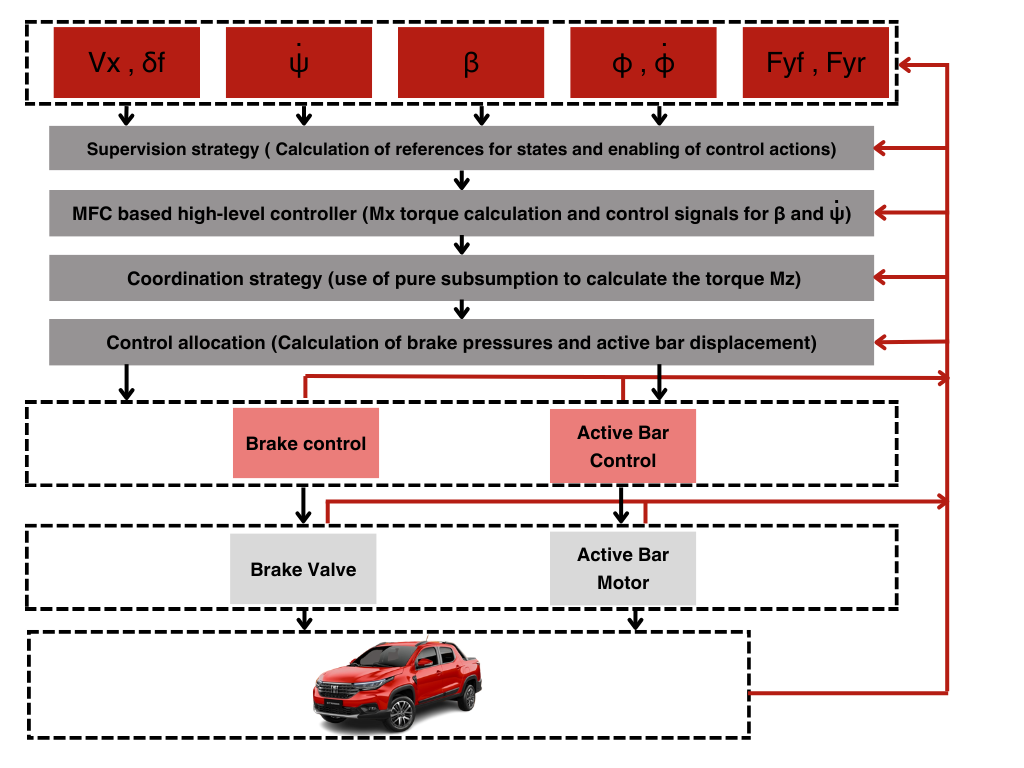
\includegraphics[width=\linewidth]{MuC mio.png}
    \caption{UCC architecture}
    \label{fig:MuC mio}
\end{figure}


\subsubsection{Supervision layer}

The supervision layer computes the references and defines the activation 
conditions for each controller channel, as formalized in 
Section~\ref{sec:references}. The $\beta$ controller is activated only 
when $|\beta| > 2^\circ$; the $\dot{\psi}$ reference is computed 
dynamically via Eq.~(\ref{Eq:yaw_ref}); and the $\phi$ reference is 
always zero.

\subsubsection{High-level controller}

The high-level controller applies three independent iPD controllers, 
one per regulated variable, to compute the virtual control moments. 
The lateral dynamics channels ($\beta$ and $\dot{\psi}$) produce a 
combined yaw moment $M_z$, while the roll channel produces a roll 
moment $M_x$. Both are subject to the saturation limits defined in 
Eqs.~(\ref{Eq:Mz_sat})--(\ref{Eq:Mx_sat}). The implementation in 
MATLAB/Simulink\textsuperscript{\textregistered} is shown in 
Fig.~\ref{Fig:UCC-implem}.

\begin{figure*}[h]
    \centering
    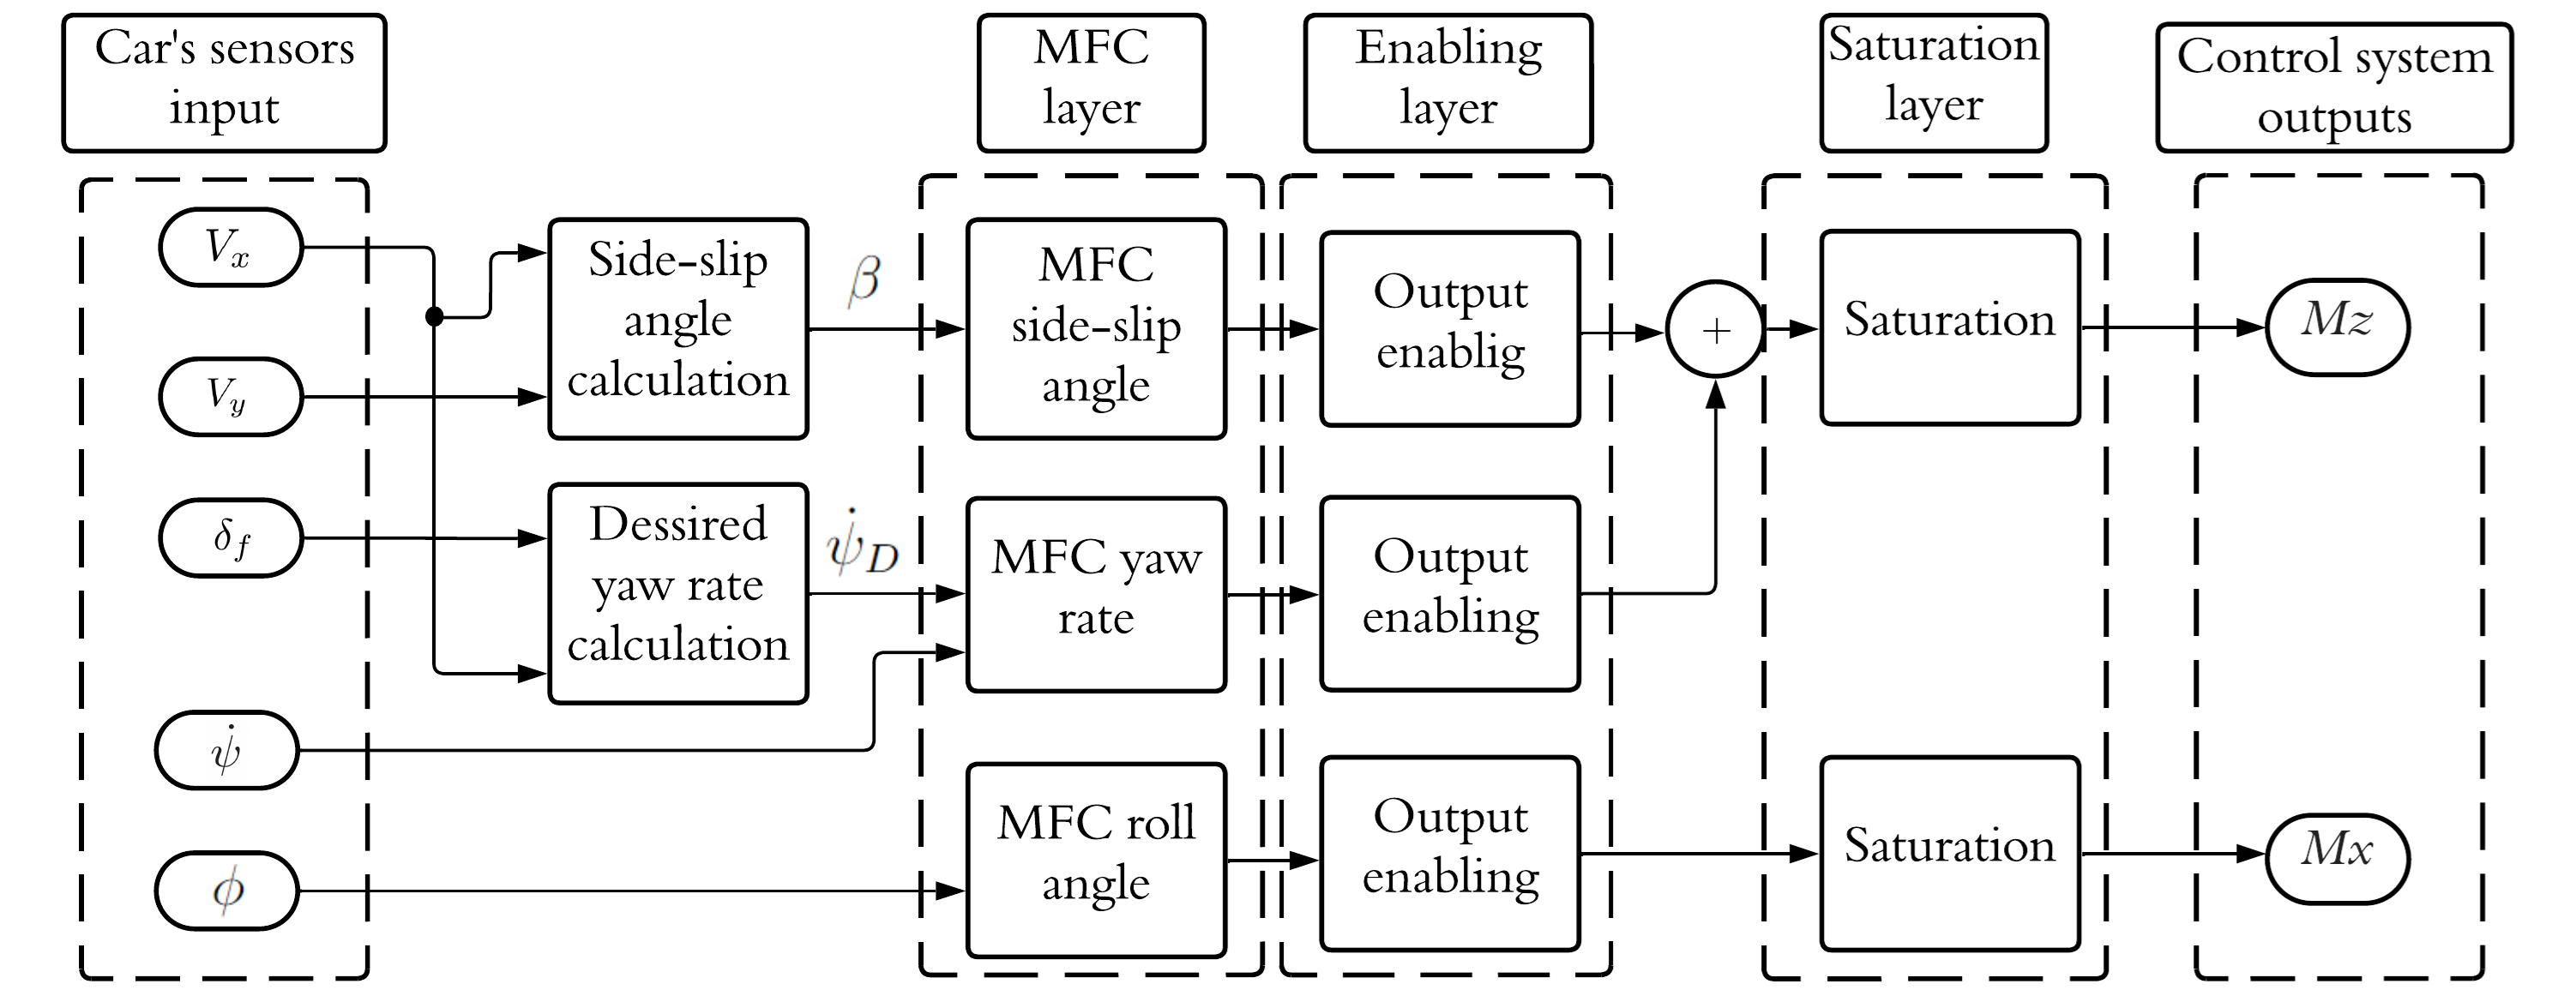
\includegraphics[width=\linewidth]{MFC_Blocos.png}
    \caption{UCC implementation}
    \label{Fig:UCC-implem}
\end{figure*}

\subsubsection{Coordination layer}

Since both the $\beta$ and $\dot{\psi}$ controllers contribute to $M_z$, 
a Pure Subsumption strategy is used in the coordination layer to weight 
their respective contributions in the final torque signal. The roll 
channel is independent and not affected by this coordination step.

% ------------------------------------------------------------------------
\subsection{Control Allocation}\label{sec:allocation}

The virtual control moments $M_z$ and $M_x$ are translated into 
physical actuator commands by CarSim\textsuperscript{\textregistered}. 
Specifically, $M_z$ is decomposed into individual wheel brake pressure 
signals processed by the ABS subsystem, and $M_x$ is converted into 
active anti-roll bar force commands. This allocation step is handled 
internally by the simulator, consistent with the setup described 
in \citep{Arronte2023}. Public CarSim documentation states that the 
built-in ESC modulates the brakes of individual wheels, but it does not 
provide the detailed internal allocation law used to map $M_z$ into 
wheel-level brake pressures, nor an explicit public description of the 
internal AARB mapping from $M_x$ to actuator commands 
\citep{carsim_builtincontrollers,carsim_fmvss126}. Accordingly, in the 
present work the allocation stage is treated as transparent to the 
high-level controller: the controller supplies the virtual moments 
$M_z$ and $M_x$, while the actuator-level distribution is resolved 
internally by CarSim.

% ------------------------------------------------------------------------
\subsection{Parameter Selection and Implementation 
            Details}\label{sec:params}

The iPD controllers involve three sets of parameters per channel: the 
scaling constant $\alpha$, the proportional gain $K_P$, and the derivative 
gain $K_D$. These were selected empirically through iterative simulation, 
guided by the following criteria: $\alpha$ was adjusted to match the 
order of magnitude of the unknown plant gain for each channel, while 
$K_P$ and $K_D$ were tuned to balance tracking performance and control 
signal smoothness, prioritizing maneuver safety over passenger comfort.

The effect of $\alpha$ on closed-loop behavior was observed to be 
monotonic: higher values introduce response delay, while lower values 
increase control signal oscillation. An intermediate value was sought 
for each channel independently. It was further verified through 
simulation that variations in $K_D$ had negligible influence on the 
system response; therefore, $K_D$ was fixed at a small value for all 
channels to provide light damping.
Although the tuning was empirical, it was guided by safety-oriented 
criteria in the SWD maneuver, namely preserving closed-loop stability, 
limiting actuator saturation, and achieving adequate transient 
regulation, whose effectiveness is confirmed by the results in 
Section~\ref{sec2}.

The resulting parameter values are summarized in 
Table~\ref{tab:params}.

\begin{table}[h]
\centering
\caption{Selected iPD parameters for each regulated channel}
\label{tab:params}
\begin{tabular}{lcccc}
\toprule
Channel & $\alpha$ & $K_P$ & $K_D$ & Ultra-local model ($v$) \\
\midrule
$\beta$ & $10^{-3}$   & $20$  & $3$ & $2$ \\
$\dot{\psi}$ & $10^{-3}$ & $50$  & $3$ & $1$ \\
$\phi$ & $10^{-2}$ & $200$ & $3$ & $2$ \\
\bottomrule
\end{tabular}
\end{table}

The simulation sampling period was set to $T_s = 1$\,ms, and the 
estimation window to $T = 1.0$\,s for all three channels.



% ------------------------------------------------------------------------
% ------------------------------------------------------------------------
% ------------------------------------------------------------------------
\section{Experimental Design} \label{sec:exper}

To validate the proposed UCC, the closed-loop system is simulated in MATLAB/Simulink\textsuperscript{\textregistered} coupled with the CarSim\textsuperscript{\textregistered} SUV model parameterized according to \cite{Arronte2023}. The experiments focus on the comparison between the proposed iPD-based MFC controller, the gain-scheduled LQR benchmark, and the open-loop vehicle response under the same test conditions, using the SWD maneuver as the common evaluation scenario. To assess robustness, three friction levels are considered \citep{Ahrenhold2023}: $\mu = 0.7$ (dry asphalt), $\mu = 0.5$ (wet road), and $\mu = 0.3$ (icy road).

The SWD maneuver involves accelerating the vehicle to a speed slightly above 80\,km/h without steering or braking, maintaining the highest gear up to 80\,km/h, and then applying a steering input in the form of a sine wave with a dwell, that is, a short hold at the maximum steering angle. The purpose of the test is to evaluate the vehicle's response to a sudden evasive maneuver, such as swerving to avoid an obstacle, in accordance with regulations such as FMVSS~126 and UN/ECE Regulation No.~13-H \cite{MSC2012}. Figure~\ref{fig:sine-maneuver} shows the steering waveform used in this study.
\begin{figure}
    \centering    
    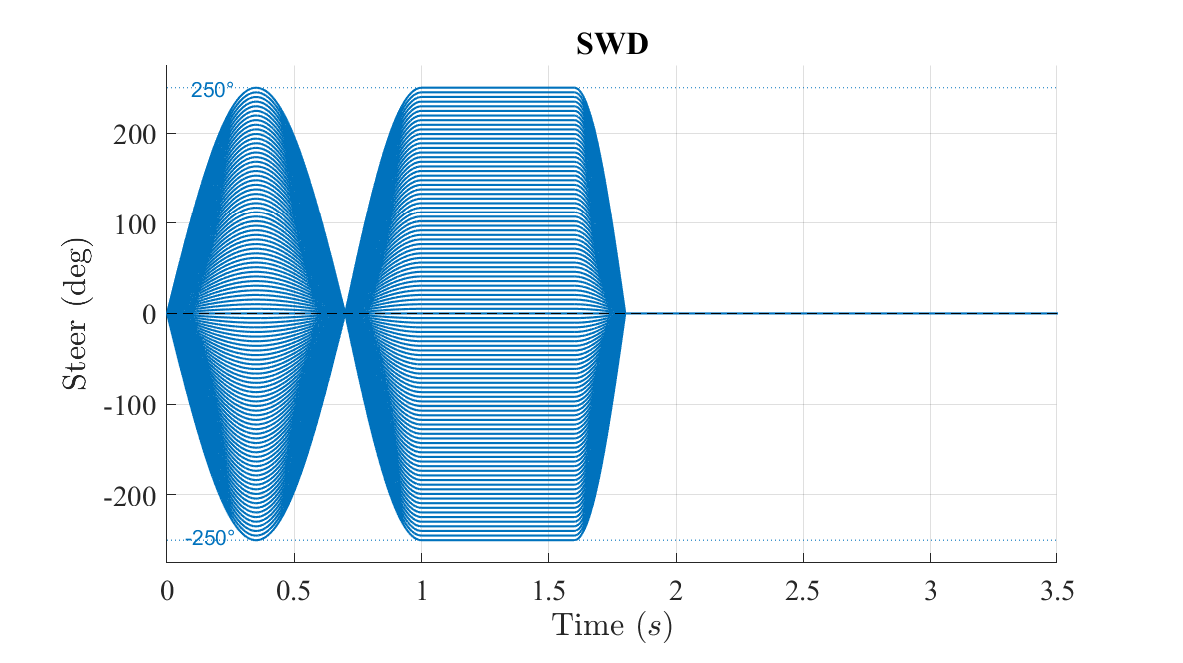
\includegraphics[width = \linewidth]{SWD_original.eps}
    \caption{Steering angle for the sine-with-dwell maneuver}
    \label{fig:sine-maneuver}
\end{figure}



% ------------------------------------------------------------------------
% ------------------------------------------------------------------------
% ------------------------------------------------------------------------
\section{Simulation Results}\label{sec2}

The UCC is evaluated through the SWD maneuver described above under three
different road-friction conditions. The results reported below compare the
open-loop vehicle response, the CarSim\textsuperscript{\textregistered}
ESC controller, the fixed-parameter 2PID+fuzzy controller, the
gain-scheduled LQR benchmark, and the proposed iPD-based MFC controller.
As will be shown, the open-loop case and the CarSim
\textsuperscript{\textregistered} ESC baseline do not guarantee stable
behavior in all tested scenarios.

%TODO: añadir una discusión más explícita sobre el alcance de la
%      estabilidad en lazo cerrado. Ahora mismo la evidencia de estabilidad
%      es esencialmente empírica y ligada a la maniobra SWD; convendría
%      precisar el dominio de validez de esa afirmación, el papel de las
%      saturaciones y qué se entiende aquí por "practical closed-loop
%      stability", en línea con la solicitud del Revisor 2.

%As a concept, a car is considered to have lateral stability in a maneuver if the side-slip angle and the difference between the measured yaw rate and the desired yaw rate are minimized. On the other hand, vertical stability (or roll stability) is achieved by minimizing the roll angle. In this work, it is not intended to minimize the roll rate (which would create a more comfortable environment for passengers) but this parameter is observed in the simulations.
 
% ------------------------------------------------------------------------
\subsection{Simulation for $\mu = 0.7$}\label{sec3}

Figures \ref{fig:beta_07} and \ref{fig:yaw_07} show the side-slip angle and yaw rate during the SWD maneuver for $\mu = 0.7$. Under this condition, both controllers, namely the gain-scheduled LQR and the iPD-based MFC, reduce the side-slip angle and keep the measured yaw rate close to its reference. By contrast, the vehicle fails to complete the maneuver in open loop. Figures \ref{fig:roll_07} and \ref{fig:roll_rate_07} show the roll angle and roll rate responses, indicating that both controllers mitigate the rollover-related dynamics during the maneuver.

%TODO: añadir al menos un zoom/inset en una figura representativa (por
%      ejemplo, alrededor del pico o de la zona donde las curvas más se
%      aproximan) para mejorar la comparación visual, tal como sugieren los
%      revisores respecto a la legibilidad de las figuras.


\begin{figure}
     \centering
     \begin{subfigure}[b]{0.4\textwidth}
         \centering
    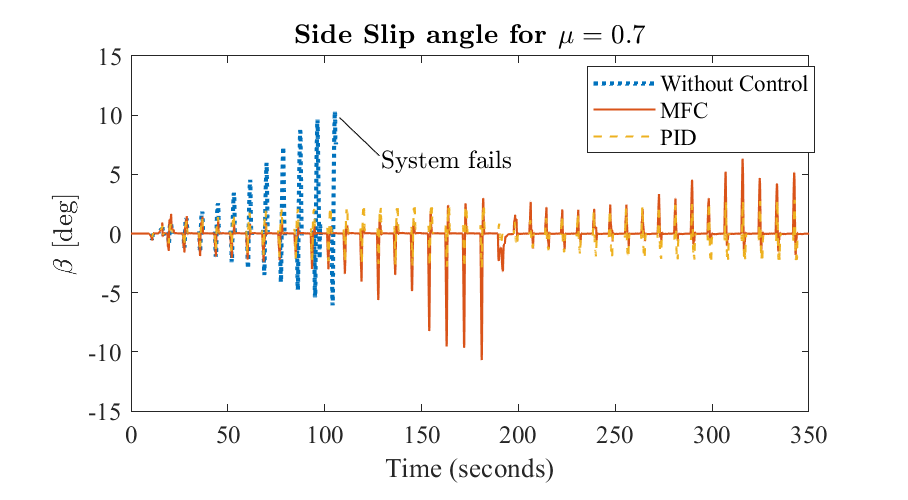
\includegraphics[width=\linewidth]{beta_07.eps}
         \caption{Side-slip angle}
         \label{fig:beta_07}
     \end{subfigure}
     \begin{subfigure}[b]{0.4\textwidth}
         \centering
    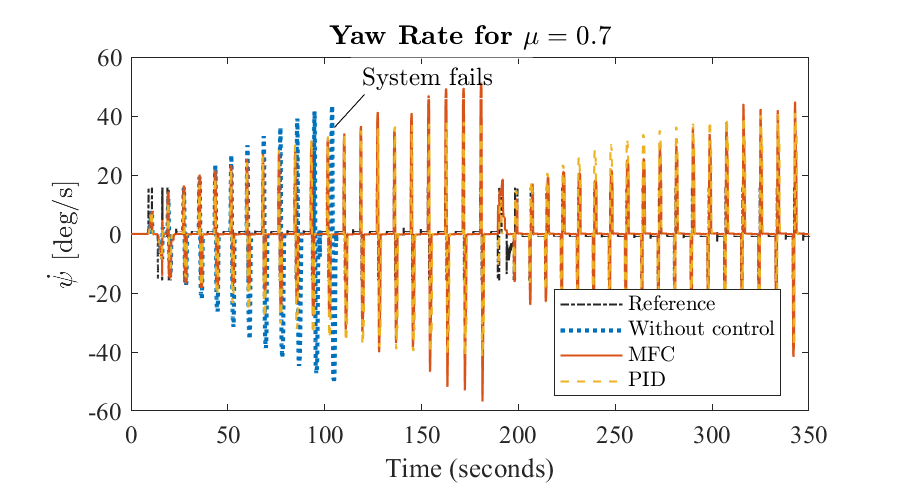
\includegraphics[width=\linewidth]{yaw_rate_07.eps}
         \caption{Yaw rate}
         \label{fig:yaw_07}
     \end{subfigure}
     \begin{subfigure}[b]{0.4\textwidth}
         \centering
    
\includegraphics[width=\linewidth]{roll_07.eps}
         \caption{Roll angle}
         \label{fig:roll_07}
     \end{subfigure}
     \begin{subfigure}[b]{0.4\textwidth}
         \centering
    
\includegraphics[width=\linewidth]{roll_rate_07.eps}
         \caption{Roll rate}
         \label{fig:roll_rate_07}
     \end{subfigure}     
        \caption{Results for $\mu = 0.7$}
        \label{fig:mu_07}
\end{figure}




% \begin{figure}[h]
%     \centering
%     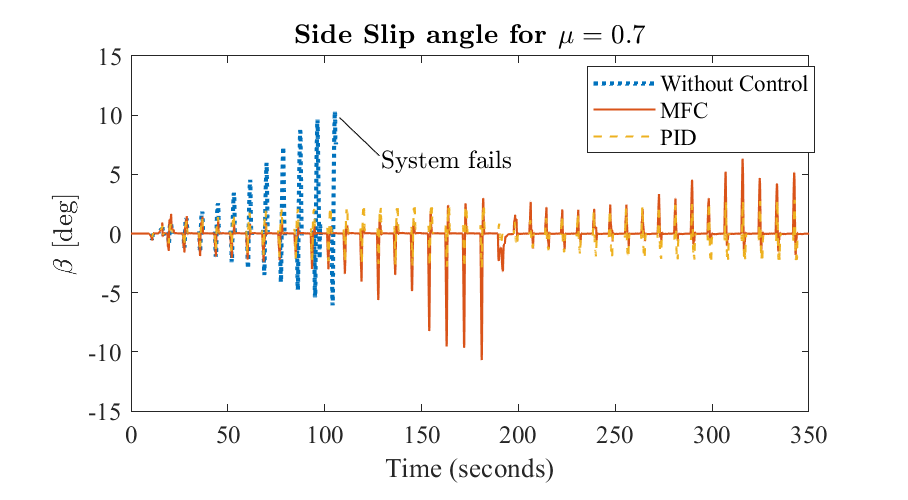
\includegraphics[width=0.7\linewidth]{beta_07.eps}
%     \caption{Side-slip angle for $\mu=0.7$}
%     \label{fig:beta_07}
% \end{figure}
% \begin{figure}[h]
%     \centering
%     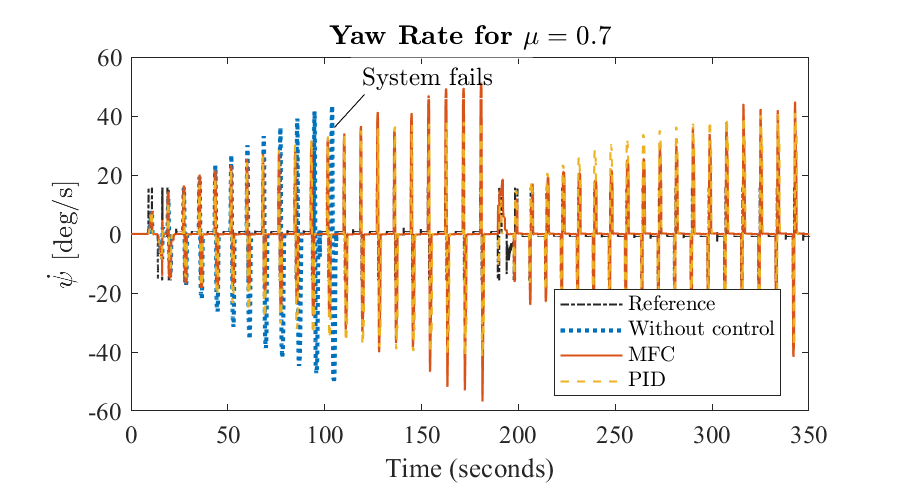
\includegraphics[width=0.7\linewidth]{yaw_rate_07.eps}
%     \caption{Yaw rate for $\mu=0.7$}
%     \label{fig:yaw_07}
% \end{figure}
% \begin{figure}[h]
%     \centering
%     
\includegraphics[width=0.7\linewidth]{roll_07.eps}
%     \caption{Roll angle for $\mu=0.7$}
%     \label{fig:roll_07}
% \end{figure}
% \begin{figure}[h]
%     \centering
%     
\includegraphics[width=0.7\linewidth]{roll_rate_07.eps}
%     \caption{Roll rate for $\mu=0.7$}
%     \label{fig:roll_rate_07}
% \end{figure}


% ------------------------------------------------------------------------
\subsection{Simulation for $\mu = 0.5$}

Figures \ref{fig:beta_05} and \ref{fig:yaw_05} show the side-slip angle and yaw rate, respectively, during the SWD maneuver with $\mu = 0.5$. Both controllers reduce the side-slip angle and keep the yaw rate close to its reference. As in the previous case, the open-loop vehicle does not complete the maneuver. Figures \ref{fig:roll_05} and \ref{fig:roll_rate_05} show the corresponding roll angle and roll rate responses, which again confirm the beneficial effect of the controllers on rollover-related dynamics.



\begin{figure}
     \centering
     \begin{subfigure}[b]{0.4\textwidth}
         \centering
    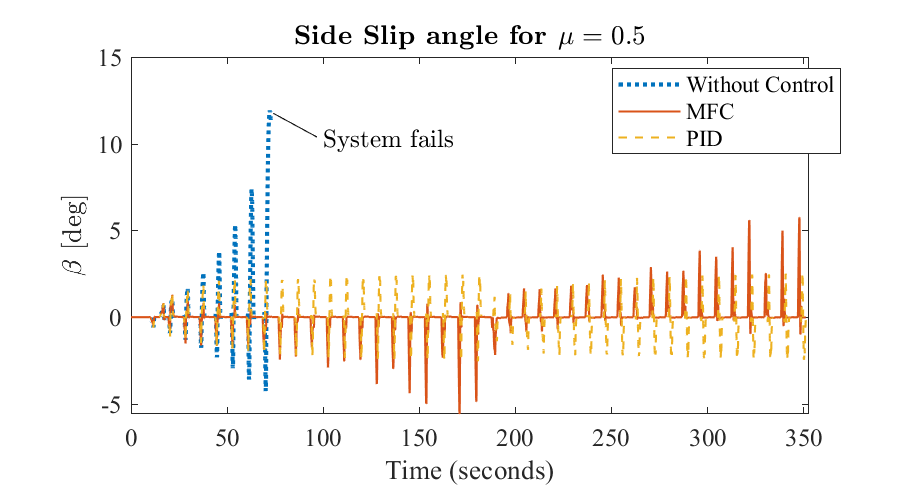
\includegraphics[width=\linewidth]{beta_05.eps}
         \caption{Side-slip angle}
         \label{fig:beta_05}
     \end{subfigure}
     \begin{subfigure}[b]{0.4\textwidth}
         \centering
    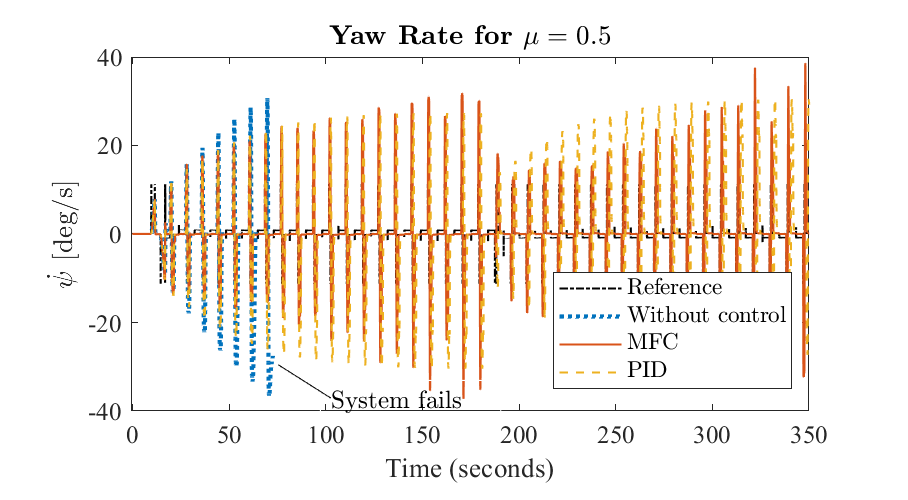
\includegraphics[width=\linewidth]{yaw_rate_05.eps}
         \caption{Yaw rate}
         \label{fig:yaw_05}
     \end{subfigure}
     \begin{subfigure}[b]{0.4\textwidth}
         \centering
    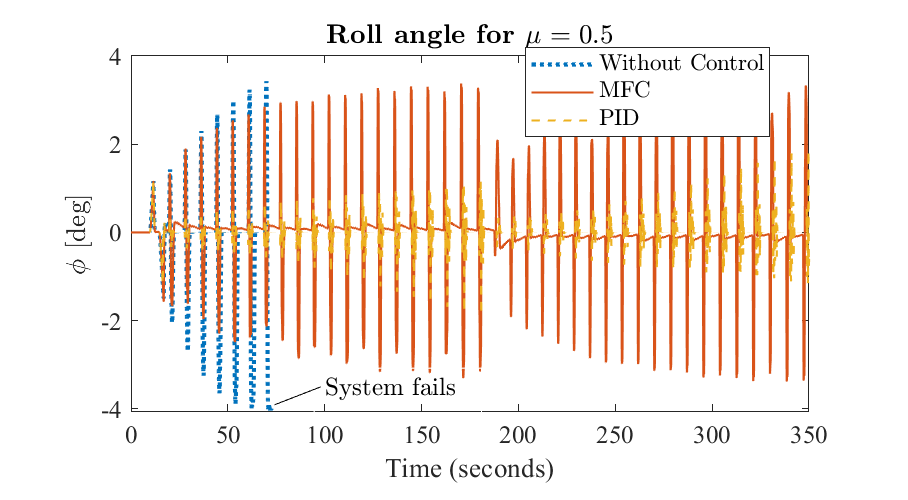
\includegraphics[width=\linewidth]{roll_05.eps}
         \caption{Roll angle}
         \label{fig:roll_05}
     \end{subfigure}
     \begin{subfigure}[b]{0.4\textwidth}
         \centering
    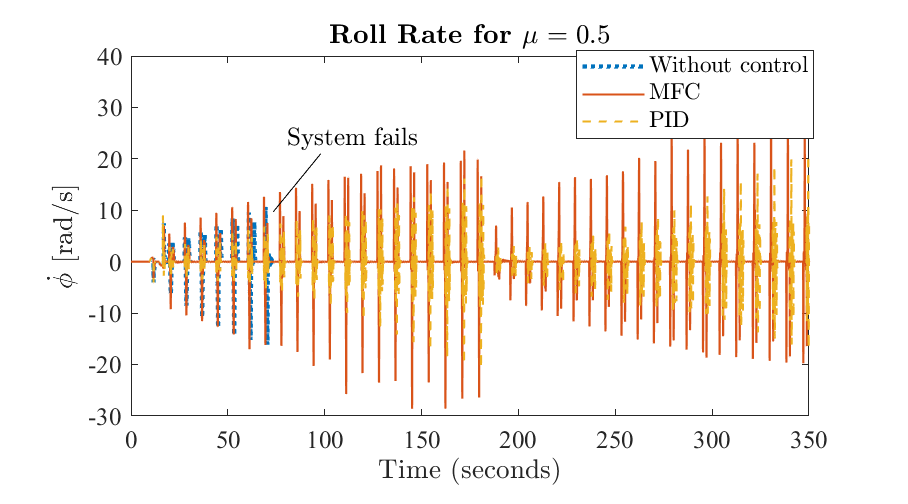
\includegraphics[width=\linewidth]{roll_rate_05.eps}
         \caption{Roll rate}
         \label{fig:roll_rate_05}
     \end{subfigure}     
        \caption{Results for $\mu = 0.5$}
        \label{fig:mu_05}
\end{figure}



% \begin{figure}[htbp]
%     \centering
%     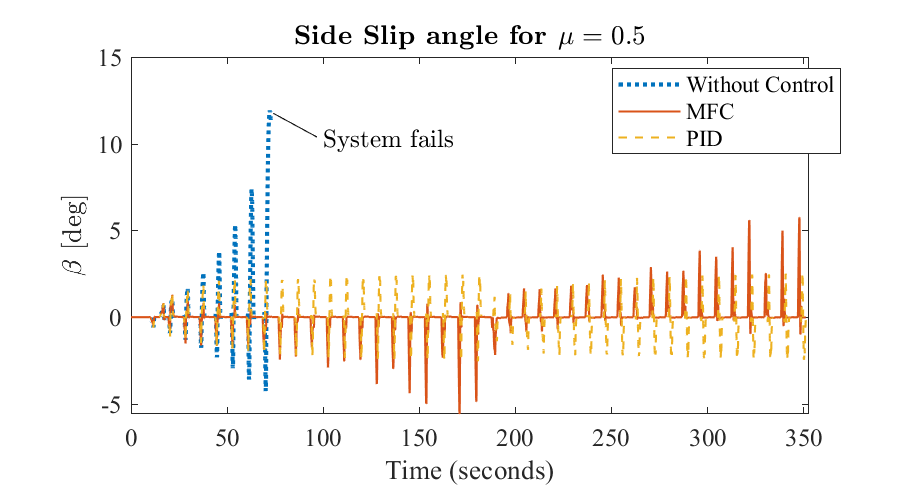
\includegraphics[width=0.7\linewidth]{beta_05.eps}
%     \caption{Side-slip angle for $\mu=0.5$}
%     \label{fig:beta_05}
% \end{figure}
% \begin{figure}[htbp]
%     \centering
%     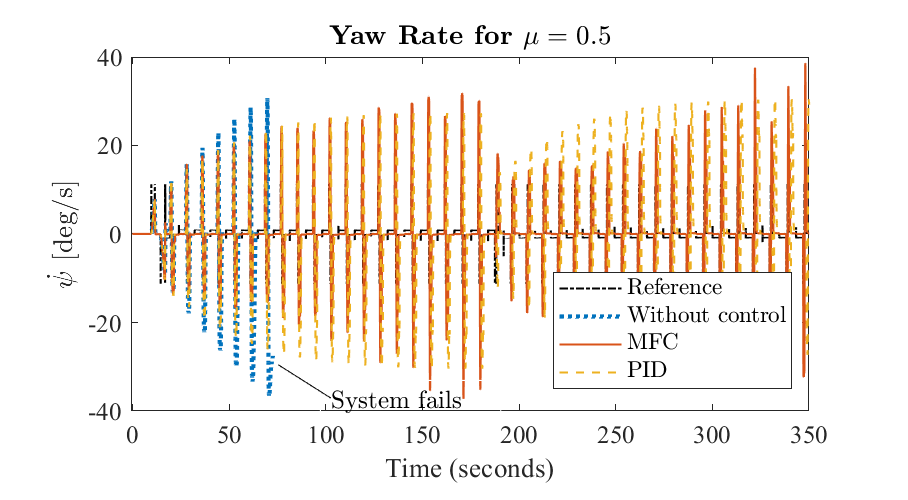
\includegraphics[width=0.7\linewidth]{yaw_rate_05.eps}
%     \caption{Yaw rate for $\mu=0.5$}
%     \label{fig:yaw_05}
% \end{figure}
% \begin{figure}[htbp]
%     \centering
%     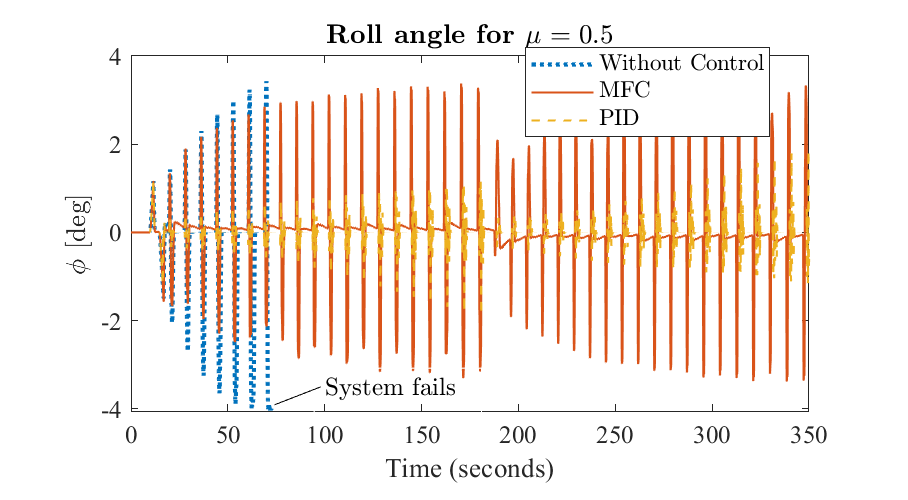
\includegraphics[width=0.7\linewidth]{roll_05.eps}
%     \caption{Roll angle for $\mu=0.5$}
%     \label{fig:roll_05}
% \end{figure}
% \begin{figure}[htbp]
%     \centering
%     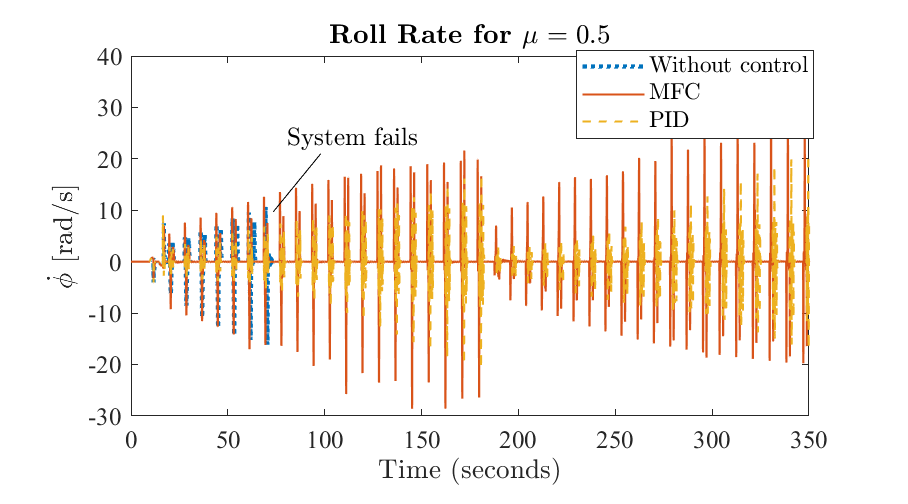
\includegraphics[width=0.7\linewidth]{roll_rate_05.eps}
%     \caption{Roll rate for $\mu=0.5$}
%     \label{fig:roll_rate_05}
% \end{figure}



% ------------------------------------------------------------------------
\subsection{Simulation for $\mu = 0.3$}

Figures \ref{fig:beta_03} and \ref{fig:yaw_03} show the side-slip angle and yaw rate, respectively, during the SWD maneuver with $\mu = 0.3$. Under this low-friction condition, only the iPD-based MFC controller is able to complete the maneuver while reducing the side-slip angle and yaw-rate tracking error. Both the open-loop case and the gain-scheduled LQR benchmark fail shortly after the maneuver begins. Figures \ref{fig:roll_03} and \ref{fig:roll_rate_03} show that the same pattern is reflected in the roll dynamics, whereas the proposed MFC controller maintains the roll response within an acceptable range.

\begin{figure}
     \centering
     \begin{subfigure}[b]{0.4\textwidth}
         \centering
    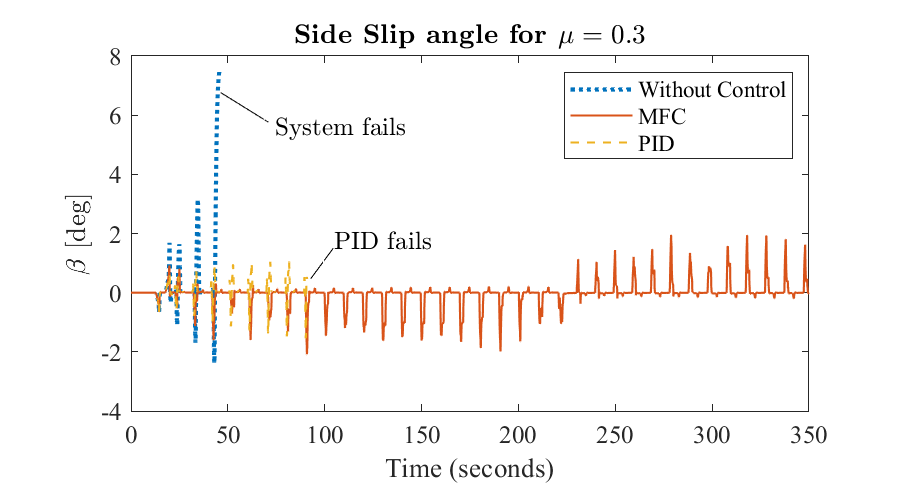
\includegraphics[width=\linewidth]{beta_03.eps}
         \caption{Side-slip angle}
         \label{fig:beta_03}
     \end{subfigure}
     \begin{subfigure}[b]{0.4\textwidth}
         \centering
    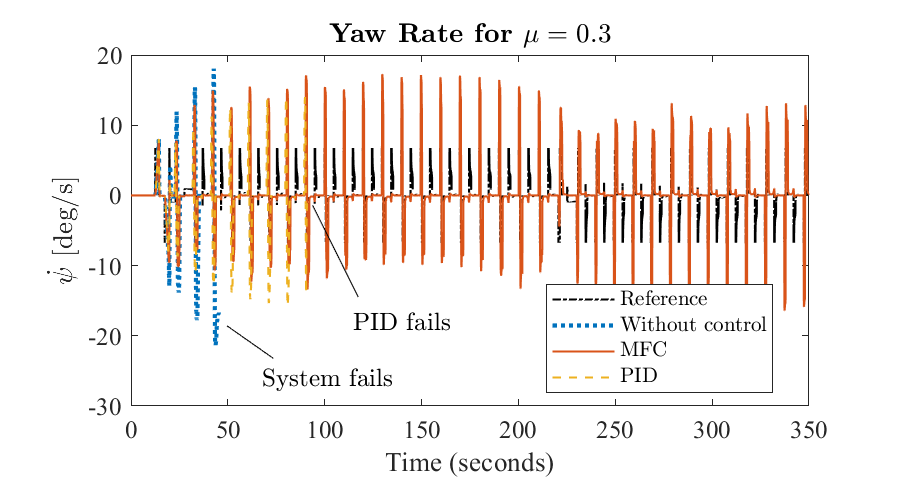
\includegraphics[width=\linewidth]{yaw_rate_03.eps}
         \caption{Yaw rate}
         \label{fig:yaw_03}
     \end{subfigure}
     \begin{subfigure}[b]{0.4\textwidth}
         \centering
    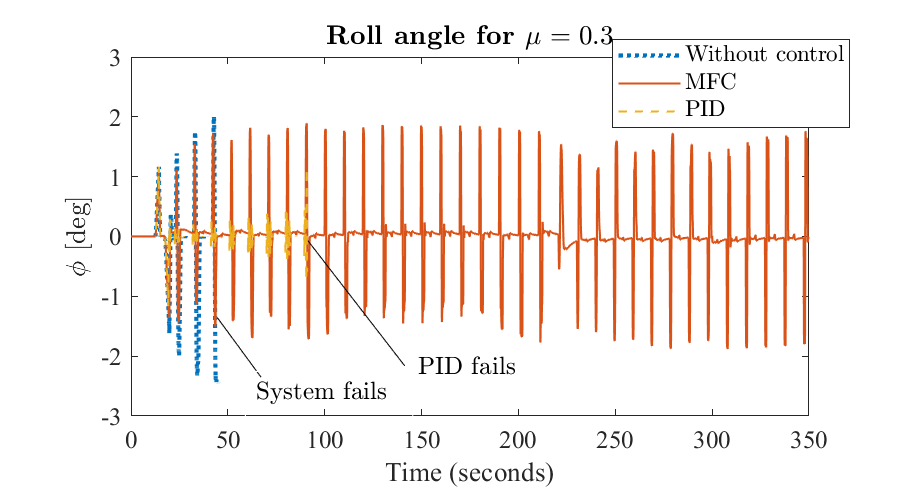
\includegraphics[width=\linewidth]{roll_03.eps}
         \caption{Roll angle}
         \label{fig:roll_03}
     \end{subfigure}
     \begin{subfigure}[b]{0.4\textwidth}
         \centering
    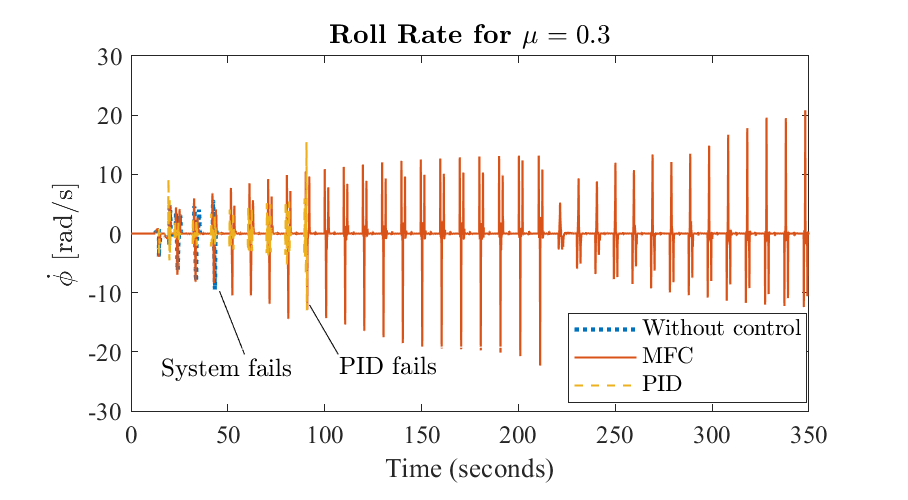
\includegraphics[width=\linewidth]{roll_rate_03.eps}
         \caption{Roll rate}
         \label{fig:roll_rate_03}
     \end{subfigure}     
        \caption{Results for $\mu = 0.3$}
        \label{fig:mu_03}
\end{figure}


% \begin{figure}[htbp]
%     \centering
%     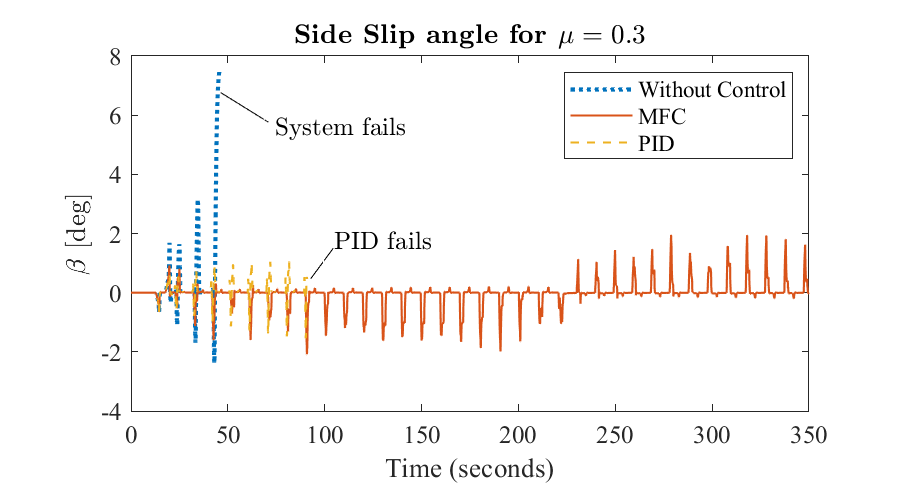
\includegraphics[width=0.7\linewidth]{beta_03.eps}
%     \caption{Side-slip angle for $\mu=0.3$}
%     \label{fig:beta_03}
% \end{figure}
% \begin{figure}[htbp]
%     \centering
%     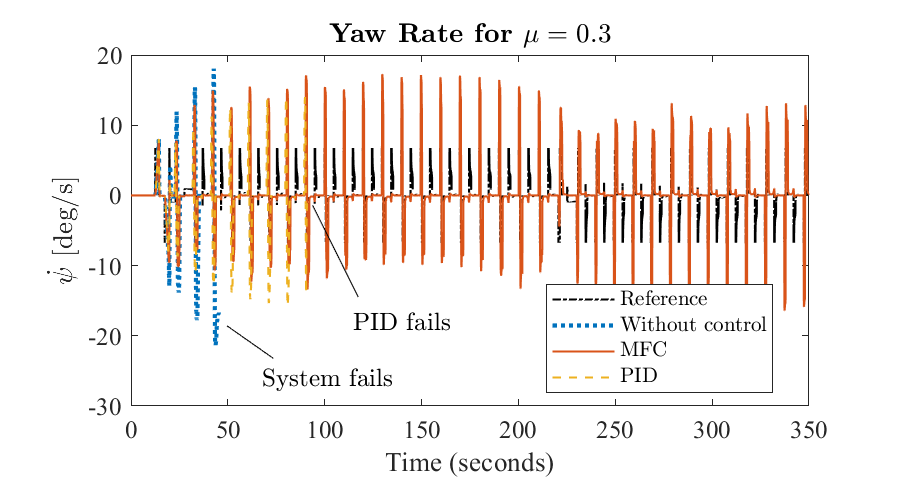
\includegraphics[width=0.7\linewidth]{yaw_rate_03.eps}
%     \caption{Yaw rate for $\mu=0.3$}
%     \label{fig:yaw_03}
% \end{figure}
% \begin{figure}[htbp]
%     \centering
%     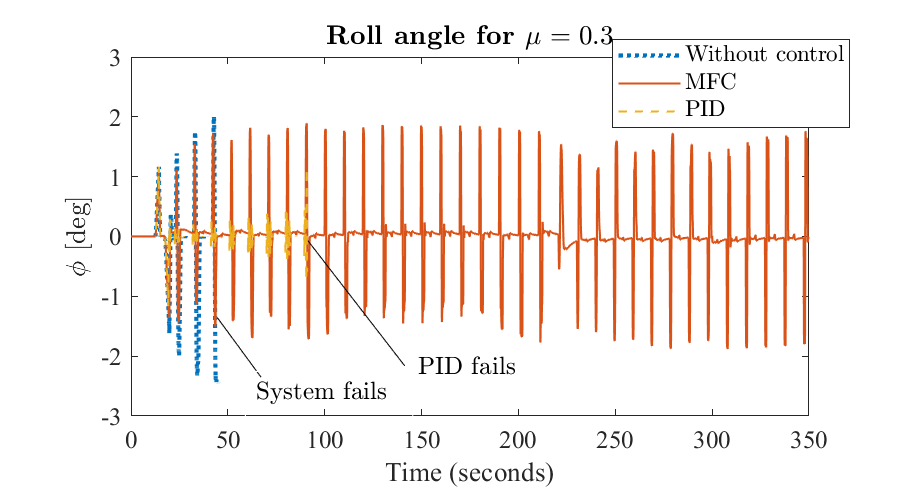
\includegraphics[width=0.7\linewidth]{roll_03.eps}
%     \caption{Roll angle for $\mu=0.3$}
%     \label{fig:roll_03}
% \end{figure}
% \begin{figure}[htbp]
%     \centering
%     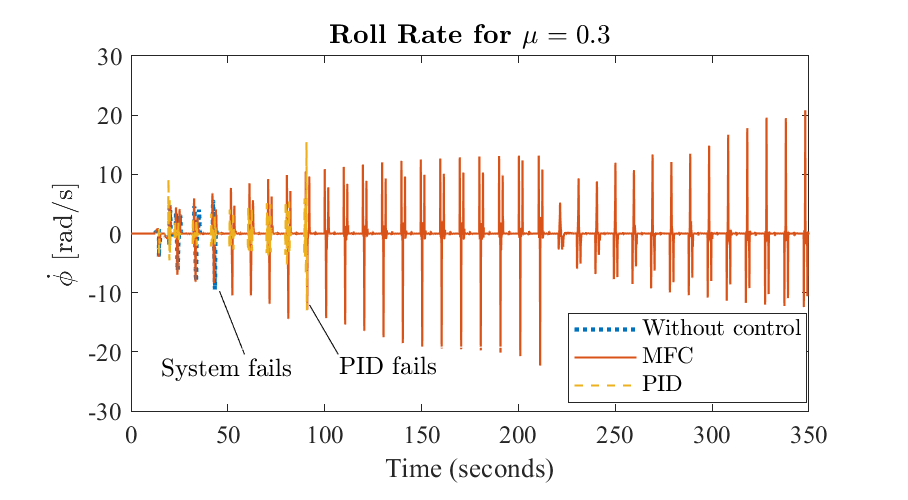
\includegraphics[width=0.7\linewidth]{roll_rate_03.eps}
%     \caption{Roll rate for $\mu=0.3$}
%     \label{fig:roll_rate_03}
% \end{figure}



% ------------------------------------------------------------------------
\subsection{Statistical results across different friction conditions}

Table~\ref{tab3} presents a statistical analysis of the vehicle's dynamic response under the SWD maneuver for the same three road friction coefficients, namely $\mu = 0.7$, $\mu = 0.5$, and $\mu = 0.3$. The results are reported for the two control strategies, gain-scheduled LQR and iPD MFC, as well as for the open-loop case. Cases in which stability is not guaranteed are highlighted in \textbf{bold}. 

\textbf{Side-slip angle:} Both controllers demonstrate a clear ability to reduce the side-slip angle. The MFC consistently achieves the lowest RMS and RMSE values, particularly at $\mu = 0.5$ and $\mu = 0.3$, where the gain-scheduled LQR benchmark shows slightly higher slip levels. At $\mu = 0.7$, MFC manages a lower RMS (0.627) compared to LQR (0.735), and at $\mu = 0.5$, this difference becomes more significant (MFC: 0.531 vs.\ LQR: 0.71). In the open-loop case, the side-slip angle increases substantially, peaking at 11.945$^\circ$ for $\mu = 0.5$, highlighting the importance of active control for maintaining lateral stability.

\textbf{Yaw rate:} In all conditions, the MFC achieves the lowest yaw rate RMS and RMSE values, followed by the gain-scheduled LQR benchmark. At $\mu = 0.7$, MFC maintains an RMS of 10.770 deg/s and a maximum yaw rate of 34.203 deg/s, while the uncontrolled vehicle reaches a peak of 49.98 deg/s. This pattern continues for $\mu = 0.5$, where MFC maintains better tracking and dampening of yaw motion. 

\textbf{Roll angle:} Roll behavior also improves with both controllers. At $\mu = 0.7$, the uncontrolled vehicle experiences an extreme peak roll angle of 79.993, while MFC and the gain-scheduled LQR limit this to 5.917$^\circ$ and 4.161$^\circ$, respectively. At $\mu = 0.5$, the LQR benchmark shows superior performance in minimizing the roll angle (RMS: 0.222), while MFC reaches a higher RMS (1.260) but still provides acceptable control.

\textbf{Roll rate:} Similar to the roll angle, the roll rate is substantially reduced by the control strategies. At $\mu = 0.7$, the uncontrolled vehicle reaches a peak roll rate of 115.104 deg/s, whereas the LQR and MFC controllers keep it below 42 deg/s. The same trend is observed for $\mu = 0.5$, with the MFC showing higher values than LQR at $\mu = 0.5$.

For $\mu = 0.3$, the gain-scheduled LQR benchmark and the open-loop case do not remain stable. Overall, the analysis demonstrates that both control strategies significantly enhance vehicle stability and rollover mitigation during the SWD maneuver for $\mu = 0.7$ and $\mu = 0.5$, with the MFC generally offering superior performance in minimizing side-slip and yaw-rate errors. The roll angle and roll rate are better controlled by the LQR benchmark. On the other hand, the iPD-based MFC exhibits greater stability robustness, since it does not fail when $\mu = 0.3$. The uncontrolled vehicle is not robustly stable. 

% \begin{table*}
% \setlength{\tabcolsep}{0.2cm}
% %\begin{sidewaystable}
% \caption{Statistical analysis of simulations}\label{tab3}
% \begin{tabular*}{\textwidth}{llccccccccc}
% \hline
% & & \multicolumn{3}{c}{GS-LQR} & \multicolumn{3}{c}{MFC} & \multicolumn{3}{c}{No Control} \\
% \cmidrule(lr){3-5}\cmidrule(lr){6-8}\cmidrule(lr){9-11}
% Parameter & $\mu$ & RMS\footnotemark[1] & RMSE\footnotemark[2] & MAX\footnotemark[3] & RMS\footnotemark[1] & RMSE\footnotemark[2] & MAX\footnotemark[3] & RMS\footnotemark[1] & RMSE\footnotemark[2] & MAX\footnotemark[3] \\
% \hline
% \multirow{3}{*}{Side-slip angle} & 0.7 & 0.735 & 0.735 & 2.889 & 0.627 & 0.627 & 3.404 & 1.826 & 1.826 & 10.33 \\
% & 0.5 & 0.71 & 0.71  & 2.531  & 0.531 & 0.531 & 2.86  & 2.074 & 2.074 & 11.945  \\
% & 0.3 & 0.280 & 0.280 & 1.54 & 0.382 & 0.382 & 2.077 & 1.387 & 1.387 & 7.466 \\
% \multirow{3}{*}{Yaw rate} & 0.7 & 12.086 & 14.751  & 40.857  & 10.770 & 13.659 & 34.203  & 12.730 & 15.165 & 49.98  \\
% & 0.5 & 9.898 & 11.561 & 30.451 & 8.288 & 10.200 & 26.169 & 10.303 & 10.303 & 36.629 \\
% & 0.3 & 4.265 & 4.265  & 15.655 & 4.739 & 5.695 & 17.267 & 6.203 & 6.203 & 21.354 \\
% \multirow{3}{*}{Roll angle} & 0.7 & 1.335 & 1.335  & 4.161  & 1.646 & 1.646 & 5.917  & 4.642 & 4.642 & 79.993  \\
% & 0.5 & 0.222 & 0.222 & 1.852 & 1.260 & 1.260 & 4.029 & 1.340 & 1.340 & 4.050 \\
% & 0.3 & 0.164 & 0.164  & 1.166  & 0.598 & 0.598 & 1.893 & 0.804 & 0.804 & 2.452 \\
% \multirow{3}{*}{Roll rate} & 0.7 & 4.092 & 4.092  & 26.348  & 5.745 & 5.745 & 41.935  & 9.844 & 9.844 & 115.104  \\
% & 0.5 & 2.488 & 2.488 & 20.689 & 4.665 & 4.665 & 37.391 & 2.799 & 2.799 & 16.156 \\
% & 0.3 & 1.181 & 1.181  & 15.443  & 2.320 & 2.320 & 22.313 & 1.528 & 1.528 & 9.482 \\
% \Xhline{2\arrayrulewidth}
% \end{tabular*}
% \footnotetext{Note: All data in the table are in the same unit as their corresponding variable. For example: an RMS corresponding to the yaw rate of a specific maneuver will be in deg/s.}
% \footnotetext[1]{Root Mean Square (related to signal).}
% \footnotetext[2]{Root Mean Square Error (related to reference).}
% \footnotetext[3]{Maximum absolute value.}
% %\end{sidewaystable}
% \end{table*}

% \begin{table*}[ht]
% \caption{Statistical analysis of simulations (lack of stability robustness highlighted in \textbf{bold})}
% \label{tab3}
% \begin{threeparttable}
% \centering
% \setlength{\tabcolsep}{5pt}
% \begin{tabular}{llccccccccc}
% \toprule
% & & \multicolumn{3}{c}{GS-LQR} & \multicolumn{3}{c}{MFC} & \multicolumn{3}{c}{No Control} \\
% \cmidrule(lr){3-5} \cmidrule(lr){6-8} \cmidrule(lr){9-11}
% Parameter & $\mu$ & RMS\tnote{1} & RMSE\tnote{2} & MAX\tnote{3} & RMS & RMSE & MAX & RMS & RMSE & MAX \\
% \midrule
% \multirow{3}{*}{Side-slip angle} 
% & 0.7 & 0.735 & 0.735 & 2.889 & 0.627 & 0.627 & 3.404 & \textbf{1.826} & \textbf{1.826} & \textbf{10.33} \\
% & 0.5 & 0.710 & 0.710 & 2.531 & 0.531 & 0.531 & 2.860 & \textbf{2.074} & \textbf{2.074} & \textbf{11.945} \\
% & 0.3 & \textbf{0.280} & \textbf{0.280} & \textbf{1.540} & 0.382 & 0.382 & 2.077 & \textbf{1.387} & \textbf{1.387} & \textbf{7.466} \\
% \midrule
% \multirow{3}{*}{Yaw rate}
% & 0.7 & 12.086 & 14.751 & 40.857 & 10.770 & 13.659 & 34.203 & \textbf{12.730} & \textbf{15.165} & \textbf{49.980} \\
% & 0.5 & 9.898 & 11.561 & 30.451 & 8.288 & 10.200 & 26.169 & \textbf{10.303} & \textbf{10.303} & \textbf{36.629} \\
% & 0.3 & \textbf{4.265} & \textbf{4.265} & \textbf{15.655} & 4.739 & 5.695 & 17.267 & \textbf{6.203} & \textbf{6.203} & \textbf{21.354} \\
% \midrule
% \multirow{3}{*}{Roll angle}
% & 0.7 & 1.335 & 1.335 & 4.161 & 1.646 & 1.646 & 5.917 & \textbf{4.642} & \textbf{4.642} & \textbf{79.993} \\
% & 0.5 & 0.222 & 0.222 & 1.852 & 1.260 & 1.260 & 4.029 & \textbf{1.340} & \textbf{1.340} & \textbf{4.050} \\
% & 0.3 & \textbf{0.164} & \textbf{0.164} & \textbf{1.166} & 0.598 & 0.598 & 1.893 & \textbf{0.804} & \textbf{0.804} & \textbf{2.452} \\
% \midrule
% \multirow{3}{*}{Roll rate}
% & 0.7 & 4.092 & 4.092 & 26.348 & 5.745 & 5.745 & 41.935 & \textbf{9.844} & \textbf{9.844} & \textbf{115.104} \\
% & 0.5 & 2.488 & 2.488 & 20.689 & 4.665 & 4.665 & 37.391 & \textbf{2.799} & \textbf{2.799} & \textbf{16.156} \\
% & 0.3 & \textbf{1.181} & \textbf{1.181} & \textbf{15.443} & 2.320 & 2.320 & 22.313 & \textbf{1.528} & \textbf{1.528} & \textbf{9.482} \\
% \bottomrule
% \end{tabular}
% \begin{tablenotes}
% \footnotesize
% \item[1] Root Mean Square (related to signal).
% \item[2] Root Mean Square Error (related to reference).
% \item[3] Maximum absolute value.
% \end{tablenotes}
% \end{threeparttable}
% \end{table*}

% \begin{sidewaystable}[!ht]
%     \centering
%     \begin{tabular}{|l|l|l|l|l|l|l|l|l|l|l|l|l|l|l|l|l|l|l|l|l|l|}
%     \hline
%         Open Loop & Carsim ESC & 2PID+Fuzzy & GS-LQR & iPID & ~ & ~ & ~ & ~ & ~ & ~ & ~ & ~ & ~ & ~ & ~ & ~ & ~ & ~ & ~ & ~ & ~ \\ \hline
%         Prameter & mu & RMS & RMSE & MAX & ST & RMS & RMSE & MAX & ST & RMS & RMSE & MAX & ST & RMS & RMSE & MAX & ST & RMS & RMSE & MAX & ST \\ \hline
%         $\beta$ & 0.3 & 1.3865 & 1.3865 & 7.4658 & 45.6040 & 4.3328 & 4.3328 & 79.9872 & 101.8755 & 0.2802 & 0.2802 & 1.5401 & 90.8950 & 84.0626 & 84.0626 & 180 & 180.0 & 0.3820 & 0.3820 & 2.0773 & 180.0 \\ \hline
%         ~ & 0.5 & 2.0735 & 2.0735 & 11.9446 & 72.7040 & 0.6085 & 0.6085 & 1.6017 & 32.8805 & 0.7095 & 0.7095 & 2.5307 & 180.0 & 1.4398 & 1.4398 & 5.5587 & 80.7220 & 0.7330 & 0.7330 & 5.7423 & 180.0 \\ \hline
%         ~ & 0.7 & 1.8257 & 1.8257 & 10.3295 & 106.0340 & 0.8429 & 0.8429 & 2.2731 & 57.8050 & 0.6793 & 0.6793 & 2.8959 & 180.0 & 2.4362 & 2.4362 & 8.4473 & 180.0 & 1.0634 & 1.0634 & 10.6926 & 180.0 \\ \hline
%         $\dot{\psi}$ & 0.3 & 6.2029 & 4.7779 & 21.3541 & 45.6040 & 112.9537 & 112.8709 & 444.0231 & 101.8755 & 4.2652 & 2.0899 & 15.6547 & 90.8950 & 161.4949 & 11025 & 559.4037 & 180.0 & 4.7386 & 2.7861 & 17.2675 & 180.0 \\ \hline
%         ~ & 0.5 & 10.3026 & 7.7189 & 36.6287 & 72.7040 & 6.8931 & 6.8115 & 22.2112 & 32.8805 & 9.8975 & 5.1593 & 30.4512 & 180.0 & 6.3843 & 12.3886 & 23.6014 & 80.7220 & 8.9371 & 5.2175 & 38.6147 & 180.0 \\ \hline
%         ~ & 0.7 & 12.7302 & 8.6956 & 49.9795 & 106.0340 & 8.5793 & 8.4799 & 30.1345 & 57.8050 & 12.0261 & 8.9794 & 41.4211 & 180.0 & 9.5523 & 17.7459 & 33.1855 & 180.0 & 12.1507 & 7.4796 & 56.7753 & 180.0 \\ \hline
%         $\phi$ & 0.3 & 0.8038 & 0.8038 & 2.4516 & 45.6040 & 10.0893 & 10.0893 & 195.4223 & 101.8755 & 0.1644 & 0.1644 & 1.1661 & 90.8950 & 5.3870 & 5.3870 & 77.7313 & 180.0 & 0.5981 & 0.5981 & 1.8932 & 180.0 \\ \hline
%         ~ & 0.5 & 1.3398 & 1.3398 & 4.0499 & 72.7040 & 1.2443 & 1.2443 & 7.1238 & 32.8805 & 0.2223 & 0.2223 & 1.8518 & 180.0 & 0.7291 & 0.7291 & 1.9372 & 80.7220 & 1.0816 & 1.0816 & 3.3769 & 180.0 \\ \hline
%         ~ & 0.7 & 4.6383 & 4.6383 & 79.9933 & 106.0340 & 1.9532 & 1.9532 & 10.1961 & 57.8050 & 0.2275 & 0.2275 & 1.8189 & 180.0 & 1.0800 & 1.0800 & 2.8552 & 180.0 & 1.4269 & 1.4269 & 5.1379 & 180.0 \\ \hline
%         $\dot{\phi}$  & 0.3 & 1.5275 & 1.5275 & 9.4818 & 45.6040 & 161.6824 & 161.6824 & 522.0664 & 101.8755 & 1.1813 & 1.1813 & 15.4329 & 90.8950 & 23.3285 & 23.3285 & 583.2962 & 180.0 & 2.3198 & 2.3198 & 22.3129 & 180.0 \\ \hline
%         ~ & 0.5 & 2.7989 & 2.7989 & 16.1562 & 72.7040 & 6.7776 & 6.7776 & 32.3786 & 32.8805 & 2.4884 & 2.4884 & 20.6892 & 180.0 & 2.0264 & 2.0264 & 14.6179 & 80.7220 & 3.7970 & 3.7970 & 31.4270 & 180.0 \\ \hline
%         ~ & 0.7 & 9.8414 & 9.8414 & 115.1039 & 106.0340 & 7.9221 & 7.9221 & 28.9968 & 57.8050 & 2.4859 & 2.4859 & 18.1210 & 180.0 & 2.9383 & 2.9383 & 21.3752 & 180.0 & 4.6610 & 4.6610 & 33.4922 & 180.0 \\ \hline
%     \end{tabular}
% \end{sidewaystable}

% \begin{sidewaystable}[!ht]
% \centering
% \small
% \begin{tabular}{llcccccccccccccccccccc}
% \toprule

% & & \multicolumn{4}{c}{Open Loop} 
%   & \multicolumn{4}{c}{Carsim ESC}
%   & \multicolumn{4}{c}{2PID+Fuzzy}
%   & \multicolumn{4}{c}{GS-LQR}
%   & \multicolumn{4}{c}{iPID} \\

% \cmidrule(lr){3-6} \cmidrule(lr){7-10} \cmidrule(lr){11-14} \cmidrule(lr){15-18} \cmidrule(lr){19-22}

% Parameter & $\mu$
% & RMS & RMSE & MAX & ST
% & RMS & RMSE & MAX & ST
% & RMS & RMSE & MAX & ST
% & RMS & RMSE & MAX & ST
% & RMS & RMSE & MAX & ST \\

% \midrule

% \multirow{3}{*}{$\beta$}
% & 0.3 & 1.3865 & 1.3865 & 7.4658 & 45.6040 & 4.3328 & 4.3328 & 79.9872 & 101.8755 & 0.2802 & 0.2802 & 1.5401 & 90.8950 & 84.0626 & 84.0626 & 180 & 180.0 & 0.3820 & 0.3820 & 2.0773 & 180.0 \\
% & 0.5 & 2.0735 & 2.0735 & 11.9446 & 72.7040 & 0.6085 & 0.6085 & 1.6017 & 32.8805 & 0.7095 & 0.7095 & 2.5307 & 180.0 & 1.4398 & 1.4398 & 5.5587 & 80.7220 & 0.7330 & 0.7330 & 5.7423 & 180.0 \\
% & 0.7 & 1.8257 & 1.8257 & 10.3295 & 106.0340 & 0.8429 & 0.8429 & 2.2731 & 57.8050 & 0.6793 & 0.6793 & 2.8959 & 180.0 & 2.4362 & 2.4362 & 8.4473 & 180.0 & 1.0634 & 1.0634 & 10.6926 & 180.0 \\

% \midrule

% \multirow{3}{*}{$\dot{\psi}$}
% & 0.3 & 6.2029 & 4.7779 & 21.3541 & 45.6040 & 112.9537 & 112.8709 & 444.0231 & 101.8755 & 4.2652 & 2.0899 & 15.6547 & 90.8950 & 161.4949 & 11025 & 559.4037 & 180.0 & 4.7386 & 2.7861 & 17.2675 & 180.0 \\
% & 0.5 & 10.3026 & 7.7189 & 36.6287 & 72.7040 & 6.8931 & 6.8115 & 22.2112 & 32.8805 & 9.8975 & 5.1593 & 30.4512 & 180.0 & 6.3843 & 12.3886 & 23.6014 & 80.7220 & 8.9371 & 5.2175 & 38.6147 & 180.0 \\
% & 0.7 & 12.7302 & 8.6956 & 49.9795 & 106.0340 & 8.5793 & 8.4799 & 30.1345 & 57.8050 & 12.0261 & 8.9794 & 41.4211 & 180.0 & 9.5523 & 17.7459 & 33.1855 & 180.0 & 12.1507 & 7.4796 & 56.7753 & 180.0 \\

% \midrule

% \multirow{3}{*}{$\phi$}
% & 0.3 & 0.8038 & 0.8038 & 2.4516 & 45.6040 & 10.0893 & 10.0893 & 195.4223 & 101.8755 & 0.1644 & 0.1644 & 1.1661 & 90.8950 & 5.3870 & 5.3870 & 77.7313 & 180.0 & 0.5981 & 0.5981 & 1.8932 & 180.0 \\
% & 0.5 & 1.3398 & 1.3398 & 4.0499 & 72.7040 & 1.2443 & 1.2443 & 7.1238 & 32.8805 & 0.2223 & 0.2223 & 1.8518 & 180.0 & 0.7291 & 0.7291 & 1.9372 & 80.7220 & 1.0816 & 1.0816 & 3.3769 & 180.0 \\
% & 0.7 & 4.6383 & 4.6383 & 79.9933 & 106.0340 & 1.9532 & 1.9532 & 10.1961 & 57.8050 & 0.2275 & 0.2275 & 1.8189 & 180.0 & 1.0800 & 1.0800 & 2.8552 & 180.0 & 1.4269 & 1.4269 & 5.1379 & 180.0 \\

% \midrule

% \multirow{3}{*}{$\dot{\phi}$}
% & 0.3 & 1.5275 & 1.5275 & 9.4818 & 45.6040 & 161.6824 & 161.6824 & 522.0664 & 101.8755 & 1.1813 & 1.1813 & 15.4329 & 90.8950 & 23.3285 & 23.3285 & 583.2962 & 180.0 & 2.3198 & 2.3198 & 22.3129 & 180.0 \\
% & 0.5 & 2.7989 & 2.7989 & 16.1562 & 72.7040 & 6.7776 & 6.7776 & 32.3786 & 32.8805 & 2.4884 & 2.4884 & 20.6892 & 180.0 & 2.0264 & 2.0264 & 14.6179 & 80.7220 & 3.7970 & 3.7970 & 31.4270 & 180.0 \\
% & 0.7 & 9.8414 & 9.8414 & 115.1039 & 106.0340 & 7.9221 & 7.9221 & 28.9968 & 57.8050 & 2.4859 & 2.4859 & 18.1210 & 180.0 & 2.9383 & 2.9383 & 21.3752 & 180.0 & 4.6610 & 4.6610 & 33.4922 & 180.0 \\

% \bottomrule
% \end{tabular}
% \caption{Performance comparison of control strategies under varying friction coefficients.}
% \end{sidewaystable}


\begin{table*}[!t]
\centering
\small
\begin{tabular}{lllccccc}
\toprule

Parameter & $\mu$ & Metric 
& Open Loop & Carsim ESC & 2PID+Fuzzy & GS-LQR & iPID \\

\midrule

\multirow{12}{*}{$\beta$}

& \multirow{4}{*}{0.3}
& RMS  & 1.3865 & 4.3328 & 0.2802 & 84.0626 & 0.3820 \\
& & RMSE & 1.3865 & 4.3328 & 0.2802 & 84.0626 & 0.3820 \\
& & MAX  & 7.4658 & 79.9872 & 1.5401 & 180     & 2.0773 \\
& & ST   & 45.6040 & 101.8755 & 90.8950 & 180.0 & 180.0 \\

& \multirow{4}{*}{0.5}
& RMS  & 2.0735 & 0.6085 & 0.7095 & 1.4398 & 0.7330 \\
& & RMSE & 2.0735 & 0.6085 & 0.7095 & 1.4398 & 0.7330 \\
& & MAX  & 11.9446 & 1.6017 & 2.5307 & 5.5587 & 5.7423 \\
& & ST   & 72.7040 & 32.8805 & 180.0 & 80.7220 & 180.0 \\

& \multirow{4}{*}{0.7}
& RMS  & 1.8257 & 0.8429 & 0.6793 & 2.4362 & 1.0634 \\
& & RMSE & 1.8257 & 0.8429 & 0.6793 & 2.4362 & 1.0634 \\
& & MAX  & 10.3295 & 2.2731 & 2.8959 & 8.4473 & 10.6926 \\
& & ST   & 106.0340 & 57.8050 & 180.0 & 180.0 & 180.0 \\

\midrule

\multirow{12}{*}{$\dot{\psi}$}

& \multirow{4}{*}{0.3}
& RMS  & 6.2029 & 112.9537 & 4.2652 & 161.4949 & 4.7386 \\
& & RMSE & 4.7779 & 112.8709 & 2.0899 & 11025 & 2.7861 \\
& & MAX  & 21.3541 & 444.0231 & 15.6547 & 559.4037 & 17.2675 \\
& & ST   & 45.6040 & 101.8755 & 90.8950 & 180.0 & 180.0 \\

& \multirow{4}{*}{0.5}
& RMS  & 10.3026 & 6.8931 & 9.8975 & 6.3843 & 8.9371 \\
& & RMSE & 7.7189 & 6.8115 & 5.1593 & 12.3886 & 5.2175 \\
& & MAX  & 36.6287 & 22.2112 & 30.4512 & 23.6014 & 38.6147 \\
& & ST   & 72.7040 & 32.8805 & 180.0 & 80.7220 & 180.0 \\

& \multirow{4}{*}{0.7}
& RMS  & 12.7302 & 8.5793 & 12.0261 & 9.5523 & 12.1507 \\
& & RMSE & 8.6956 & 8.4799 & 8.9794 & 17.7459 & 7.4796 \\
& & MAX  & 49.9795 & 30.1345 & 41.4211 & 33.1855 & 56.7753 \\
& & ST   & 106.0340 & 57.8050 & 180.0 & 180.0 & 180.0 \\

\midrule

\multirow{12}{*}{$\phi$}

& \multirow{4}{*}{0.3}
& RMS  & 0.8038 & 10.0893 & 0.1644 & 5.3870 & 0.5981 \\
& & RMSE & 0.8038 & 10.0893 & 0.1644 & 5.3870 & 0.5981 \\
& & MAX  & 2.4516 & 195.4223 & 1.1661 & 77.7313 & 1.8932 \\
& & ST   & 45.6040 & 101.8755 & 90.8950 & 180.0 & 180.0 \\

& \multirow{4}{*}{0.5}
& RMS  & 1.3398 & 1.2443 & 0.2223 & 0.7291 & 1.0816 \\
& & RMSE & 1.3398 & 1.2443 & 0.2223 & 0.7291 & 1.0816 \\
& & MAX  & 4.0499 & 7.1238 & 1.8518 & 1.9372 & 3.3769 \\
& & ST   & 72.7040 & 32.8805 & 180.0 & 80.7220 & 180.0 \\

& \multirow{4}{*}{0.7}
& RMS  & 4.6383 & 1.9532 & 0.2275 & 1.0800 & 1.4269 \\
& & RMSE & 4.6383 & 1.9532 & 0.2275 & 1.0800 & 1.4269 \\
& & MAX  & 79.9933 & 10.1961 & 1.8189 & 2.8552 & 5.1379 \\
& & ST   & 106.0340 & 57.8050 & 180.0 & 180.0 & 180.0 \\

\midrule

\multirow{12}{*}{$\dot{\phi}$}

& \multirow{4}{*}{0.3}
& RMS  & 1.5275 & 161.6824 & 1.1813 & 23.3285 & 2.3198 \\
& & RMSE & 1.5275 & 161.6824 & 1.1813 & 23.3285 & 2.3198 \\
& & MAX  & 9.4818 & 522.0664 & 15.4329 & 583.2962 & 22.3129 \\
& & ST   & 45.6040 & 101.8755 & 90.8950 & 180.0 & 180.0 \\

& \multirow{4}{*}{0.5}
& RMS  & 2.7989 & 6.7776 & 2.4884 & 2.0264 & 3.7970 \\
& & RMSE & 2.7989 & 6.7776 & 2.4884 & 2.0264 & 3.7970 \\
& & MAX  & 16.1562 & 32.3786 & 20.6892 & 14.6179 & 31.4270 \\
& & ST   & 72.7040 & 32.8805 & 180.0 & 80.7220 & 180.0 \\

& \multirow{4}{*}{0.7}
& RMS  & 9.8414 & 7.9221 & 2.4859 & 2.9383 & 4.6610 \\
& & RMSE & 9.8414 & 7.9221 & 2.4859 & 2.9383 & 4.6610 \\
& & MAX  & 115.1039 & 28.9968 & 18.1210 & 21.3752 & 33.4922 \\
& & ST   & 106.0340 & 57.8050 & 180.0 & 180.0 & 180.0 \\

\bottomrule
\end{tabular}
\caption{Performance comparison of control strategies under varying friction coefficients.}
\end{table*}

\begin{table*}[!t]
\centering
\footnotesize
\begin{tabular}{lllccccc}
\toprule

Parameter & $\mu$ & Metric
& Carsim ESC & 2PID+Fuzzy & GS-LQR & iPID \\

\midrule

\multirow{15}{*}{Pbs}

& \multirow{5}{*}{0.3}
& RMS        & 23.4196 & 2.6088 & 2.2192 & 8.2063 \\
& & MAX        & 55.2815 & 11.8114 & 1.68E+03 & 23.9273 \\
& & Energy     & 55876 & 618.5951 & 1.77E+03 & 2.42E+04 \\
& & Sat        & NA & 0 & 0.01 & 6.7227 \\
& & Rate RMS   & 557.7514 & 218.6228 & 3.14E+03 & 7.83E+03 \\

& \multirow{5}{*}{0.5}
& RMS        & 2.8170 & 4.9124 & 0.3941 & 6.5678 \\
& & MAX        & 12 & 66.7595 & 96.0468 & 23.9273 \\
& & Energy     & 260.9212 & 8.51E+03 & 12.5355 & 1.51E+04 \\
& & Sat        & NA & 1.5661 & 0.0056 & 1.6008 \\
& & Rate RMS   & 93.5817 & 861.0666 & 557.3531 & 5.97E+03 \\

& \multirow{5}{*}{0.7}
& RMS        & 3.4939 & 5.0176 & 0.7799 & 7.3820 \\
& & MAX        & 12 & 22.9088 & 405.6450 & 23.9273 \\
& & Energy     & 705.6629 & 8.94E+03 & 121.6541 & 1.93E+04 \\
& & Sat        & NA & 3.7111 & 0.0037 & 2.9302 \\
& & Rate RMS   & 151.9735 & 572.9802 & 1.10E+03 & 9.06E+03 \\

\midrule

\multirow{15}{*}{Mx}

& \multirow{5}{*}{0.3}
& RMS        & 492.0474 & 897.7965 & 1.55E+03 & 206.0696 \\
& & MAX        & 2228 & 3.39E+03 & 1.09E+04 & 962.1785 \\
& & Energy     & 2.13E+10 & 7.33E+07 & 8.67E+08 & 1.53E+07 \\
& & Sat        & NA & 12.5566 & 22.0652 & 0 \\
& & Rate RMS   & 764.1464 & 5.93E+03 & 9.26E+03 & 3.95E+03 \\

& \multirow{5}{*}{0.5}
& RMS        & 210.4468 & 1.98E+03 & 148.8898 & 351.4349 \\
& & MAX        & 525.3417 & 6.74E+03 & 669.5755 & 1200 \\
& & Energy     & 1.46E+06 & 1.38E+09 & 1.79E+06 & 4.34E+07 \\
& & Sat        & NA & 22.9564 & 0 & 0.2259 \\
& & Rate RMS   & 386.8675 & 9.40E+03 & 617.4531 & 7.32E+03 \\

& \multirow{5}{*}{0.7}
& RMS        & 271.0004 & 2.42E+03 & 243.2953 & 455.9170 \\
& & MAX        & 731.5411 & 9.18E+03 & 835.7442 & 1200 \\
& & Energy     & 2.94E+06 & 2.07E+09 & 1.18E+07 & 7.37E+07 \\
& & Sat        & NA & 22.3799 & 0 & 4.52 \\
& & Rate RMS   & 539.0644 & 9.85E+03 & 841.1845 & 8.04E+03 \\

\bottomrule
\end{tabular}
\caption{Control effort comparison in terms of brake pressure (Pbs) and anti-roll torque (Mx).}
\end{table*}
\section{Conclusions} \label{sec:concl}




% This study introduced a novel Unified Chassis Control (UCC) system based on Model-Free Controllers (MFCs) to simultaneously regulate the lateral (side-slip angle and yaw rate) and vertical (roll angle) dynamics of a vehicle during abrupt maneuvers. By leveraging an ultra-local model and algebraic estimators, the proposed MFC-based UCC eliminates the reliance on detailed vehicle models, addressing the challenges posed by parametric uncertainties and nonlinear dynamics inherent in traditional model-based approaches.

% The performance of the MFC-based UCC was evaluated through a Sine With Dwell (SWD) maneuver in a co-simulation environment using MATLAB/Simulink and CarSim, under varying road friction conditions ($\mu = 0.7$, 0.5, and 0.3). The results demonstrated that the MFC-based UCC effectively minimized the side-slip angle, reduced yaw rate errors, and maintained roll angle stability, ensuring both lateral and vertical vehicle stability. Notably, the MFC outperformed the gain-scheduled LQR benchmark in challenging low-friction conditions ($\mu = 0.3$), where the LQR-controlled and uncontrolled systems failed to complete the maneuver. This highlights the robustness of the MFC approach in handling adverse driving scenarios, such as icy roads, which are critical for enhancing vehicle safety.

% The successful integration of three independent MFC controllers within a multi-layer coordination architecture underscores the potential of model-free strategies for real-time vehicle control. By empirically tuning the control parameters, the system achieved a balance between responsiveness and stability, prioritizing vehicle safety over passenger comfort during sudden maneuvers. These findings contribute to the growing body of research on advanced vehicle control systems and align with global efforts to reduce traffic accidents.

% Despite these advancements, future work is needed to address certain limitations. The empirical tuning process could be enhanced with automated optimization techniques to improve precision and scalability. Additionally, real-world implementation on physical vehicles is essential to validate the system’s performance under diverse environmental conditions and hardware constraints. Comparative studies with other model-free approaches, such as neural network-based or fuzzy logic controllers, could further elucidate the advantages and trade-offs of the proposed MFC strategy. Finally, extending the UCC to include longitudinal dynamics or adaptive control for varying vehicle types (e.g., electric or heavy-duty vehicles) could broaden its applicability.

% In summary, the proposed MFC-based UCC represents a promising step toward robust and adaptable vehicle control systems, offering a viable solution for improving automotive safety and stability in critical driving scenarios. This work lays a foundation for further exploration of model-free control techniques in the pursuit of safer and more reliable transportation systems.

This study proposes a novel Unified Chassis Control (UCC) system based on Model-Free Controllers (MFCs) to simultaneously regulate vehicle lateral (side-slip angle and yaw rate) and vertical (roll angle) dynamics during abrupt maneuvers. By leveraging ultra-local models and algebraic estimators, the MFC-based UCC eliminates the need for detailed vehicle modeling, effectively addressing challenges posed by parametric uncertainties and the nonlinear nature of traditional model-based approaches. The controller was evaluated through an SWD maneuver in a co-simulation environment using MATLAB/Simulink\textsuperscript{\textregistered} and CarSim\textsuperscript{\textregistered}, under varying road friction conditions ($\mu = 0.7$, $\mu = 0.5$, and $\mu = 0.3$), and compared against a gain-scheduled LQR benchmark. Results showed that the MFC-based UCC significantly reduced side-slip angle and yaw-rate errors while maintaining good roll-angle stability, ensuring comprehensive lateral and vertical control. In low-friction scenarios ($\mu = 0.3$), only the MFC remained stable. 

Future research should focus on automating the tuning using optimization to enhance scalability and precision, validating the approach through real-world implementations, and comparing it with alternative model-free techniques such as neural networks or fuzzy logic controllers. Additionally, extending the UCC framework to account for longitudinal dynamics or adapting it for diverse vehicle types, including electric and heavy-duty platforms, could further expand its applicability. 

% ========================================================================
% INFO PARA ELIMINAR / LIMPIEZA FINAL
% 1. Revisar la conveniencia de mantener \subsection{UCC model-based}
%    y \subsection{Uncertainty Compensation}, ya que parte de ese material
%    se solapa con la Introduction y con la discusión del estado del arte.
% 2. El bloque legacy que comienza en \section{The ultra-local model-based
%    MFC controller} y sigue con \section{UCC structure} y
%    \section{Control tuning} duplica secciones activas ya presentes más
%    arriba (\ref{sec:ulmodel}, \ref{sec:ucc}, \ref{sec:allocation},
%    \ref{sec:params}) y es la causa de varias multiply-defined labels.
%    Debe eliminarse una vez se confirme que no queda contenido único por
%    rescatar de esa versión antigua.
% 3. Eliminar las figuras comentadas antiguas para $\mu=0.7$, $\mu=0.5$
%    y $\mu=0.3$ si se mantiene la versión con subfiguras.
% 4. Eliminar la tabla comentada antigua de resultados estadísticos
%    (la versión previa de Table~\ref{tab3}) si la versión actual con
%    threeparttable es la definitiva.
% 5. Eliminar los párrafos comentados de Conclusions si ya no se van a
%    reutilizar en la versión final.


\bmhead{Acknowledgements}

The authors thank Funda\c{c}\~ao de Desenvolvimento da Pesquisa - Fundep Mover - Linha V, for the Grants ``Sistema de Suspens\~ao Semi-ativa para Controle Avan\c{c}ado de Estabilidade (SUSP-EST)'' and ``Projeto, Implementa\c{c}\~ao e Testes de Componentes e Dispositivos para o Desenvolvimento de Sistemas de Assist\^encia \`a Condu\c{c}\~ao (SEGCOM)'', and Coordena\c{c}\~ao de Aperfei\c{c}oamento de Pessoal de N\'ivel Superior - Brasil (CAPES) - Finance Code 001.




\bibliography{sn-bibliography}% common bib file
%% if required, the content of .bbl file can be included here once bbl is generated
%%\input sn-article.bbl

\end{document}
